\documentclass[12pt,a4paper]{article}
\usepackage[utf8]{inputenc}
\usepackage[T1]{fontenc}
\usepackage{amsmath}
\usepackage{amsfonts}
\usepackage{amssymb}
\usepackage{graphicx}
\usepackage[left=2cm,right=2cm,top=2cm,bottom=2cm]{geometry}
\author{KONDI Abdoul malik \\ NGANDEU NDJEUKAM Alhasan}
\title{Manuelle d'utilisation de l'application de gestion de la médiathèque}
\begin{document}
\maketitle
\tableofcontents
\newpage

\section{Préambule}
Ce manuel d'utilisation ci explique comment utilisé le site web de la médiathèque afin
de permettre aux personnels de la médiathèque de ce familiariser avec ce dernier.

\newpage
\section{Se connecter à l'application}
Pour se connecter à l'application, cliquer sur le bouton se connecter.\\
Une nouvelle page vient d'apparaître. Renseigner votre e mail et votre mot de passe 
puis cliquer sur le bouton \textbf{SE CONNECTER}. C'est tous maintenant vous êtes 
connecté.

\newpage
\section{Accès au menu déroulant}
Accéder au menu déroulant comme suit : 
\subsection{Étape 1} 
\begin{itemize}
\item[•] Cliquer sur les trois barres en haut à gauche 
\end{itemize}
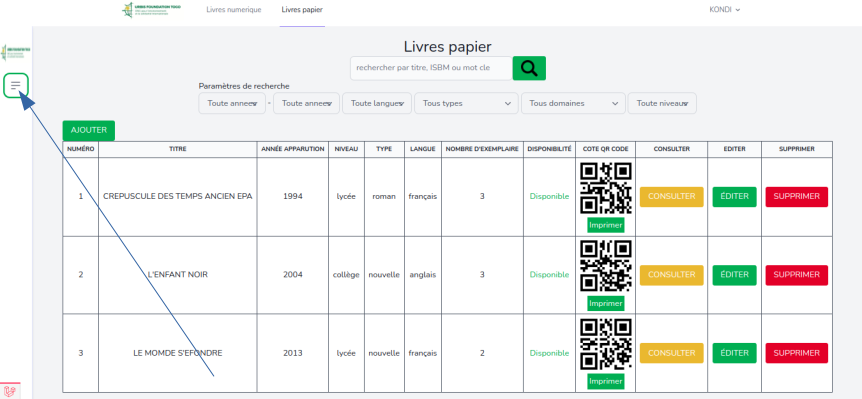
\includegraphics[scale=0.5]{images/SelectOuvragePhysique.png}

\subsection{Etape 2}
\begin{itemize}
\item[•] Après avoir cliquer sur les trois barres vous obtiendrais le résultat ci-dessous
\end{itemize}
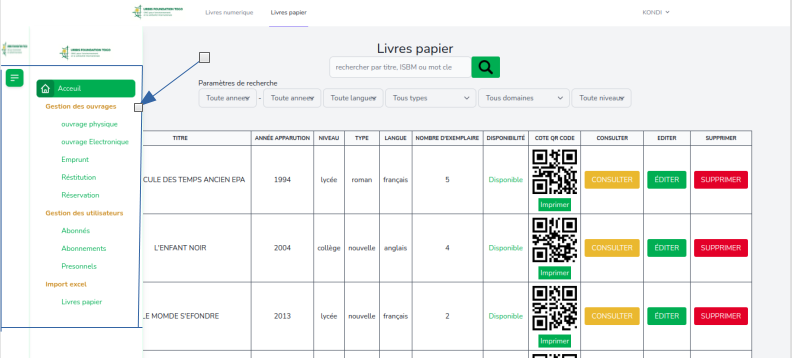
\includegraphics[scale=0.7]{images/TableauDeBord.png}.\\
Après cette étape vous pouvez sélectionner les options et les utiliser.\\
Débutons avec la \textbf{Gestion des ouvrages}.

\newpage
\section{Gestion des ouvrages}
Le menu gestion des ouvrages nous permet de gérer tous les types d'ouvrages à savoir les ouvrages physiques comme électroniques. De même la gestion des ouvrages nous permet de gérer les emprunts et restitutions.
Allons dans le menu déroulant et choisissons le menu ouvrages physiques. \\
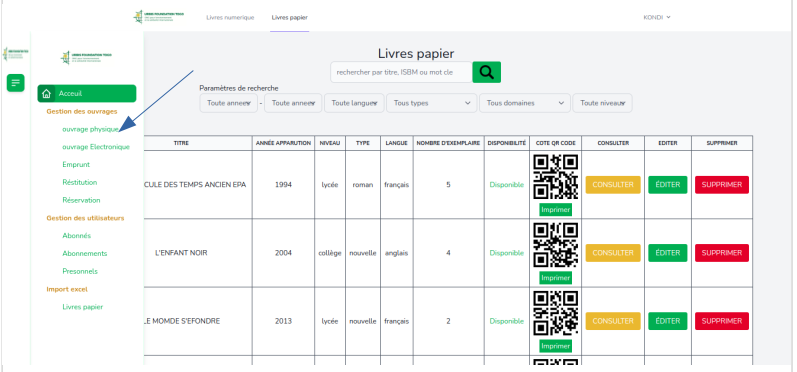
\includegraphics[scale=0.7]{images/TableauDeBord2.png}

\subsection{Accès à l'ouvrage physique}
Menu Ouvrage physique.\\

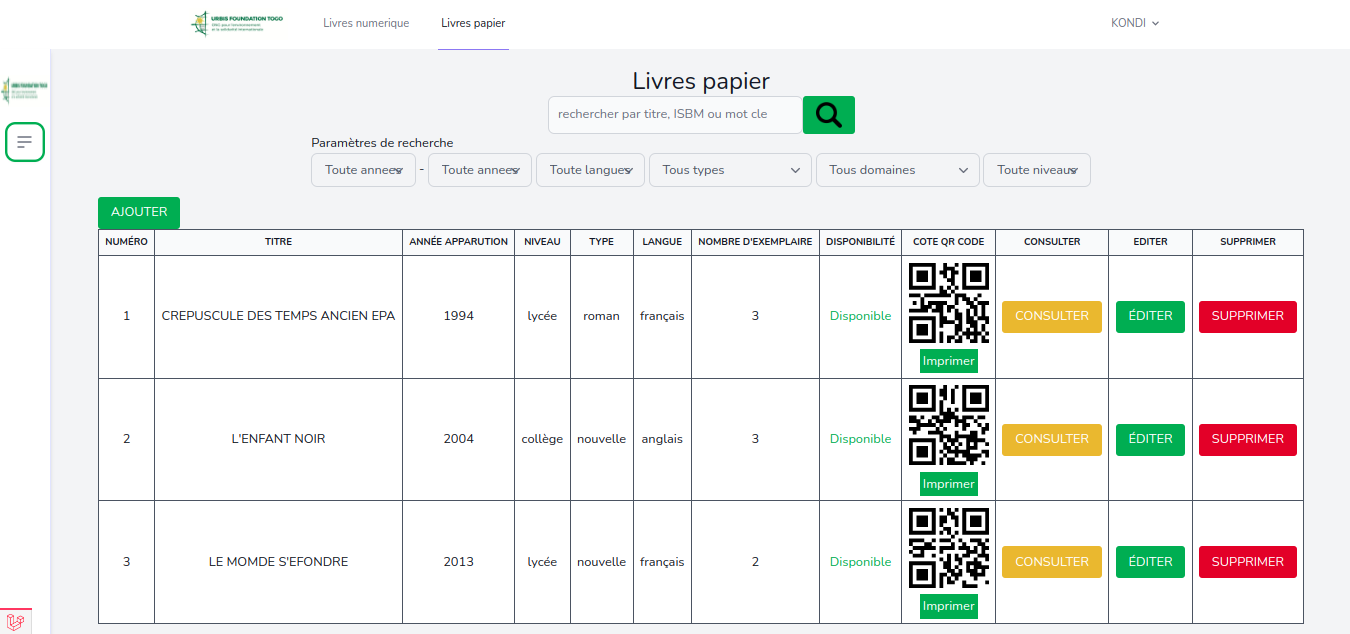
\includegraphics[scale=0.35]{images/SelectOuvragesPhysique.png}. \\

Dans le menu ouvrage physique nous pouvons ajouter un ouvrage, l'éditer, le consulter ou le supprimer.

\begin{itemize}
\item[•]Etape 1: Ajoutons un ouvrage physique.
\end{itemize}

Pour ce faire nous allons cliquer sur le boutons \textbf{ajouter} 

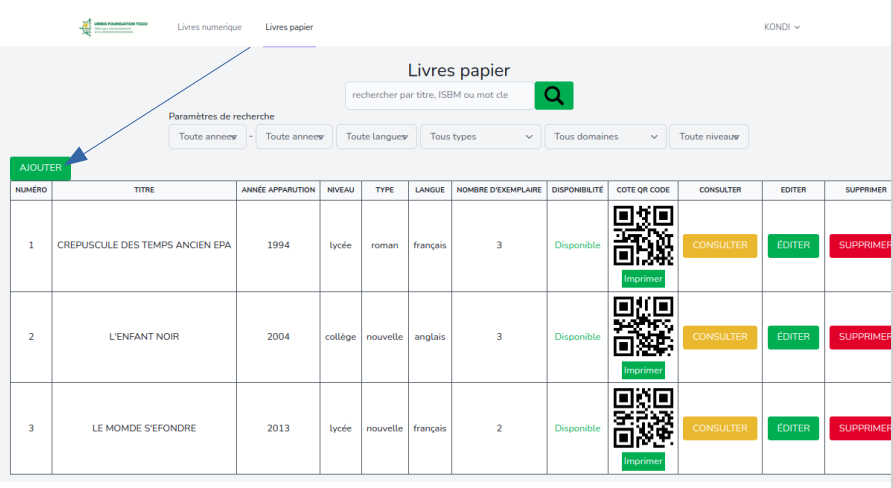
\includegraphics[scale=0.5]{images/SelectOuvragesPhysique2.png}. \\

\begin{itemize}
\item[•]Etape 2 : Remplissez les champs suivant avec des données conformes.
\end{itemize}

Comme champs à remplir nous avons :\\
\textbf{La section Ouvrage} qui contient le titre de l'ouvrage, l'image de l'ouvrage, le niveau de l'ouvrage, son type, la langue, année d'apparition et le lieu d’édition.\\
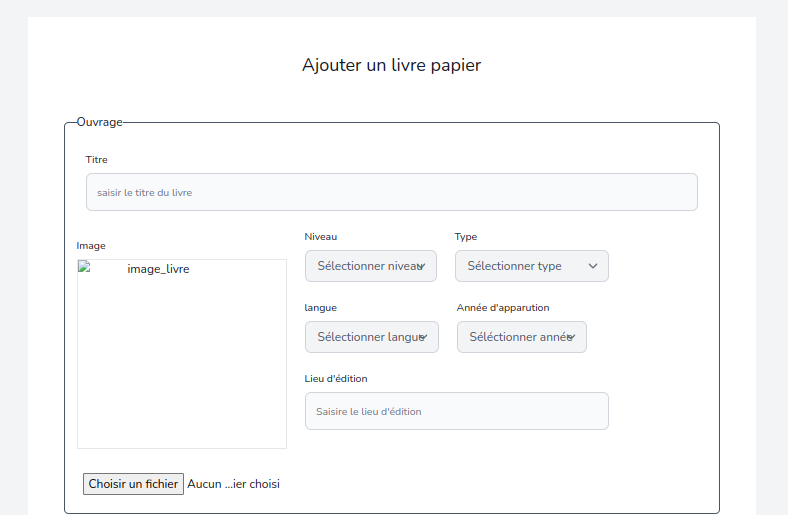
\includegraphics[scale=0.5]{images/AjoutOuvrage.png}.\\
\newpage

\textbf{La section Auteur} qui contient le nom et prénom de ou des auteurs.\\
\textbf{La section Particularité} qui contint la catégorie de l'ouvrage ainsi que l'ISBN.\\
\textbf{La section Mot clé} qui contient les mots clé de l'ouvrage. \\

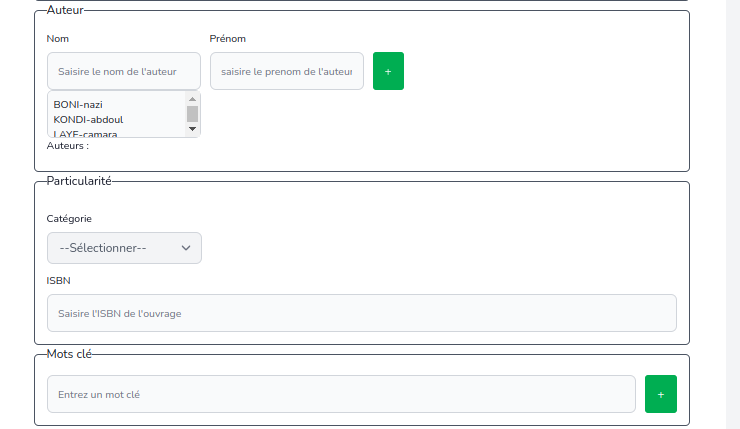
\includegraphics[scale=0.5]{images/AuteurParticulariteMotCle.png}.\\

\textbf{La section Résumé de l'ouvrage} qui contient le résumé de l'ouvrage.\\
\textbf{La section stock} qui contient le nombre d'exemplaire à la disposition de la bibliothèque, le rayon ainsi que l'étagère où se situe l'ouvrage.\\

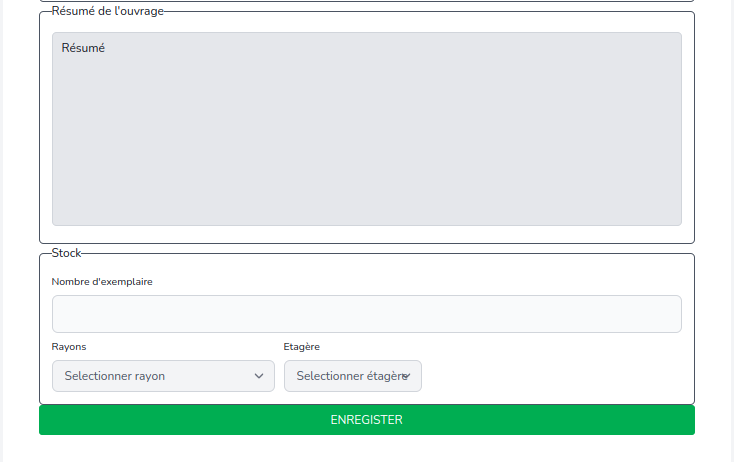
\includegraphics[scale=0.5]{images/ResumeStock.png}.\\

\textbf{Après avoir entré toute les informations vous cliquez sur le boutons enregistrer afin de valider les informations entrée}.\\

\newpage
\textbf{Dans la gestion des ouvrages vous pouvez consulter les ouvrages en cliquant sur le bouton consulté}. \\

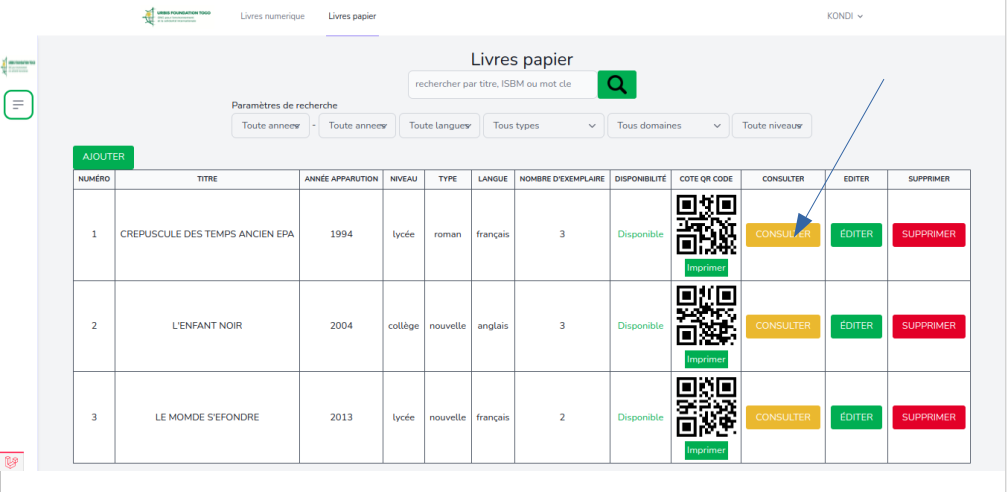
\includegraphics[scale=0.5]{images/ConsultationOuvragePhysique.png}.

Lorsque vous cliquez sur consulter vous avez la possibilité de voir les détails de l'ouvrage et vous pouvez également réserver cet ouvrage s'il n'es pas encore pris.\\

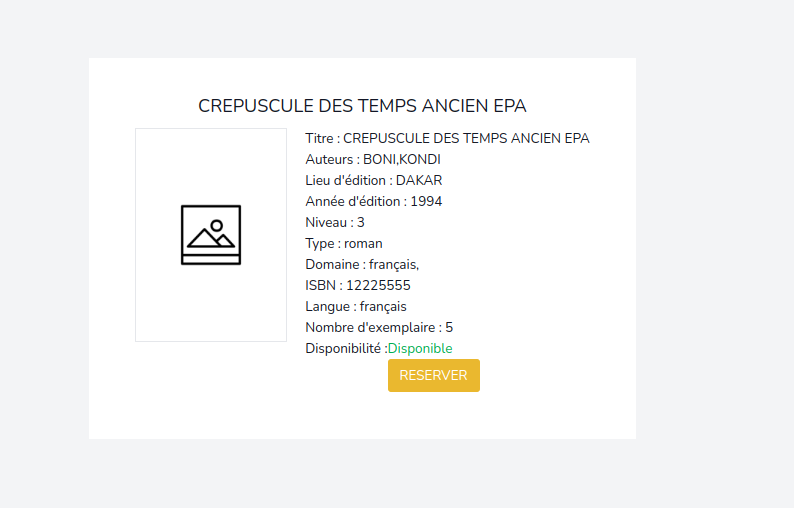
\includegraphics[scale=0.5]{images/ResulConsulter.png}.\\

\newpage

\textbf{Dans le cas où vous avez mal enregistré un ouvrage vous pouvez le modifier en cliquant sur le bouton éditer}.\\

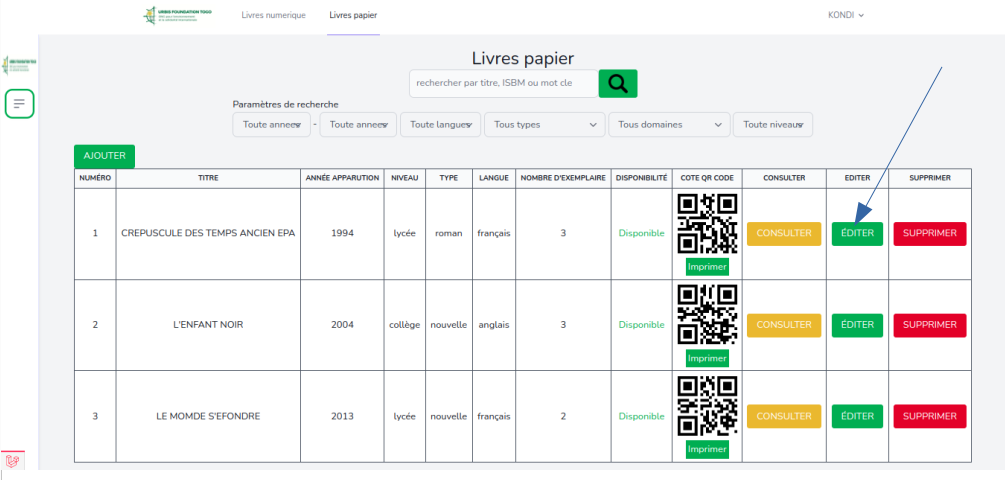
\includegraphics[scale=0.5]{images/ResulEdit.png}.\\

Ainsi lorsque vous cliquez sur éditer vous aller vous retrouver à la page d'édition qui ressemble beaucoup à celle de l'ajout d'un ouvrage mais la seule différence est que les données seront déjà rempli et vous n'avez juste qu'à les modifier. \\

\textbf{La dernière possibilité est la suppression d'un ouvrage}
Pour ce faire vous n'avez juste qu'à cliquer sur le bouton supprimer et l'ouvrage sera automatiquement supprimé.\\

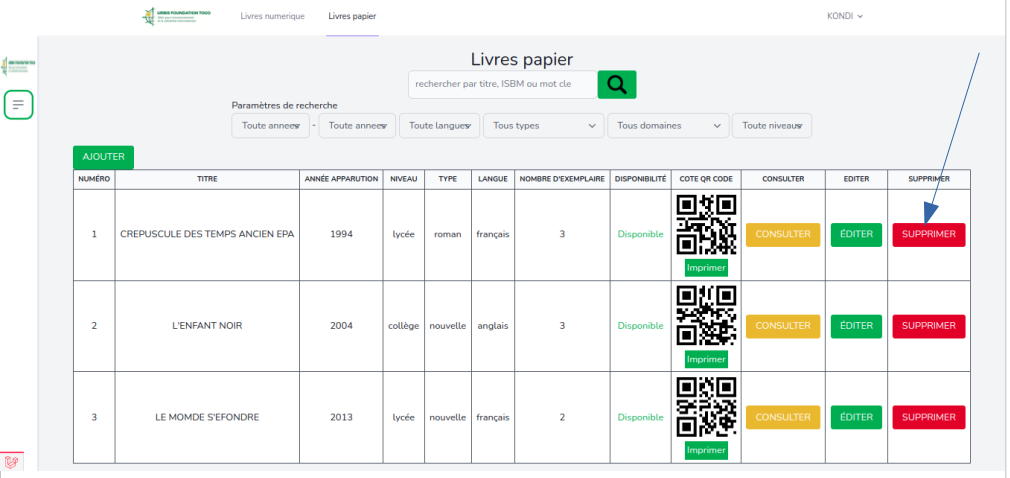
\includegraphics[scale=0.5]{images/ResulSuppression.png}.\\

\newpage
\subsection{Accès à l'Ouvrage Électronique}
Menu Ouvrage Électronique.\\
Dans un premier temps accéder au menu gestion des ouvrages puis ensuite sélectionner ouvrage électronique.\\
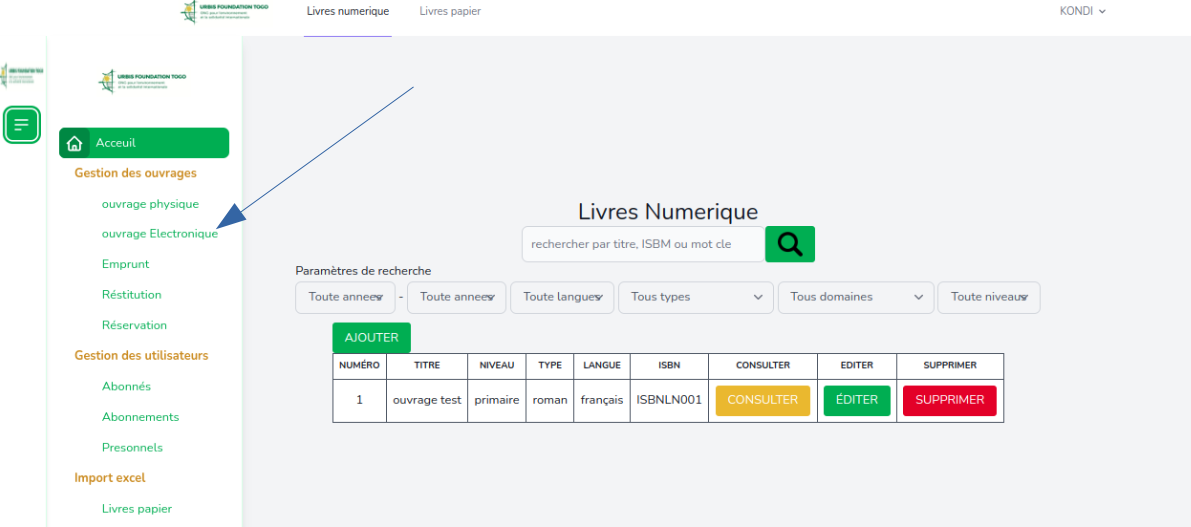
\includegraphics[scale=0.4]{images/OuVELectro.png}.\\

Après avoir cliquer nous serons sur le menu ouvrage électronique.\\

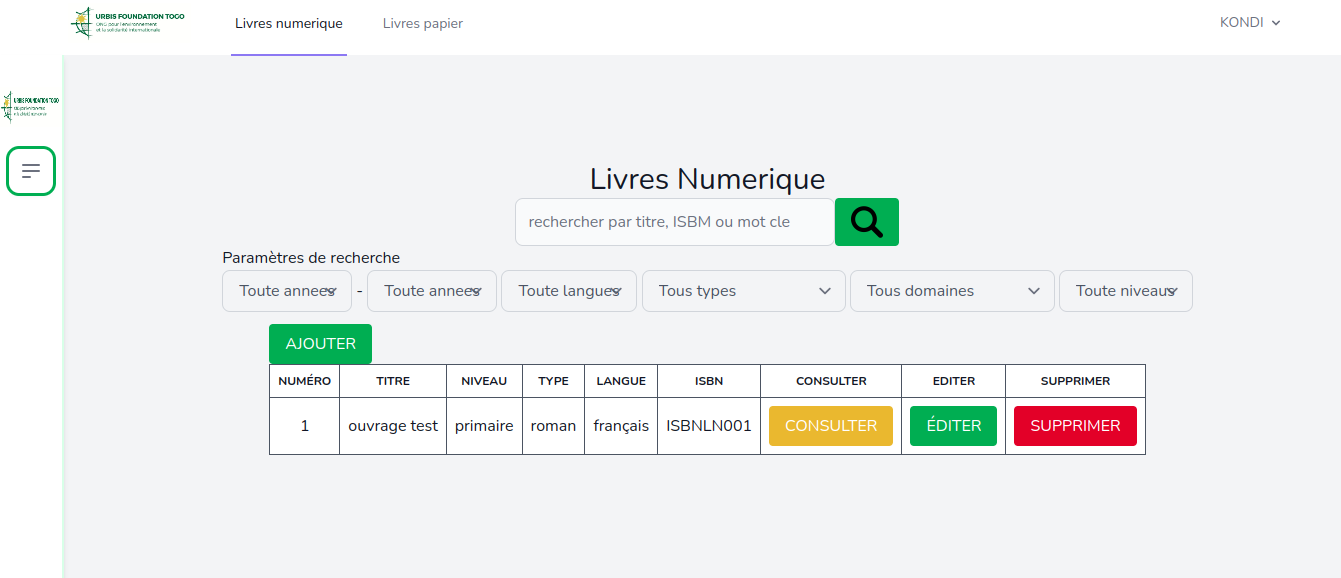
\includegraphics[scale=0.4]{images/TashBoardElectro.png}.\\

Dans le menu ouvrage électronique nous pouvons ajouter un ouvrage, l'éditer, le consulter ou le supprimer.

\begin{itemize}
\item[•]Etape 1: Ajoutons un ouvrage électronique.
\end{itemize}

Pour ce faire nous allons cliquer sur le boutons \textbf{ajouter} 

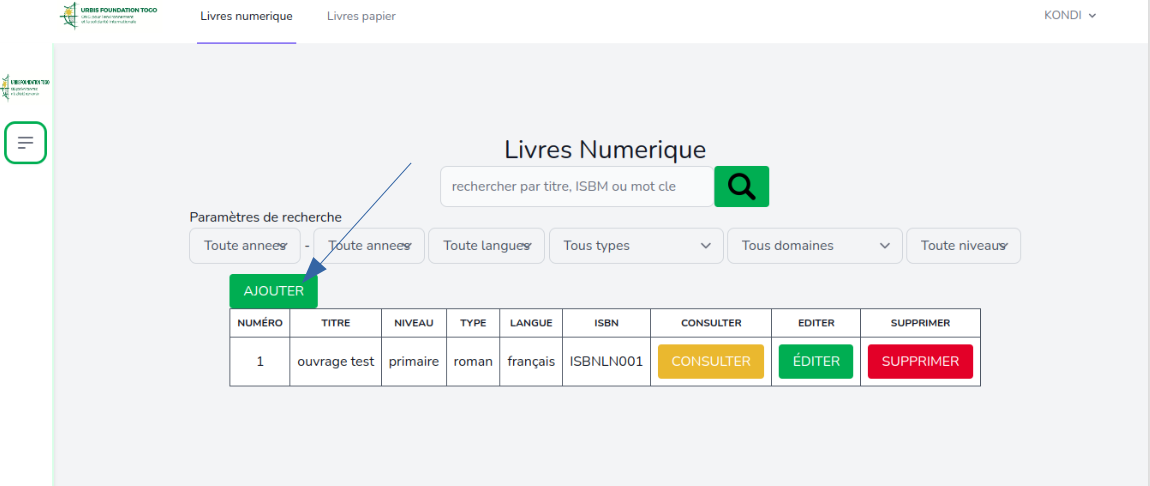
\includegraphics[scale=0.5]{images/BoutonsAjout.png}. \\

\begin{itemize}
\item[•]Etape 2 : Remplissez les champs suivant avec des données conformes.
\end{itemize}

Comme champs à remplir nous avons :\\
\textbf{La section Ouvrage} qui contient le titre de l'ouvrage, l'image de l'ouvrage, le niveau de l'ouvrage, son type, la langue, année d'apparition et le lieu d’édition.\\
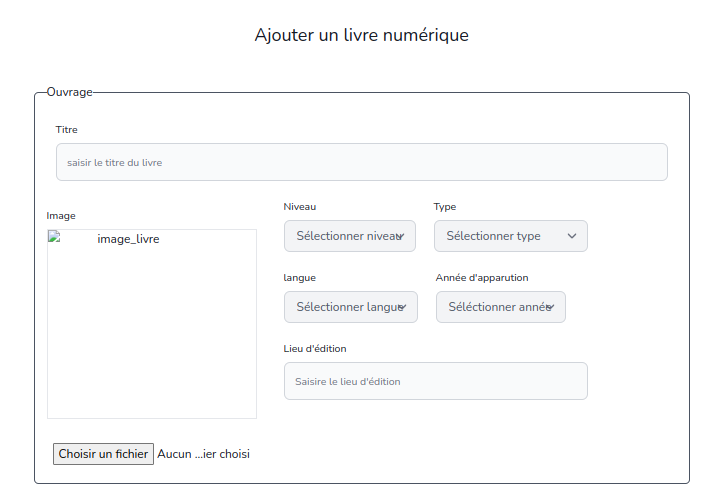
\includegraphics[scale=0.5]{images/Ajoutuvragelectro.png}.\\
\newpage

\textbf{La section Auteur} qui contient le nom et prénom de ou des auteurs.\\
\textbf{La section Particularité} qui contint la catégorie de l'ouvrage ainsi que l'ISBN.\\
\textbf{La section Mot clé} qui contient les mots clé de l'ouvrage. \\

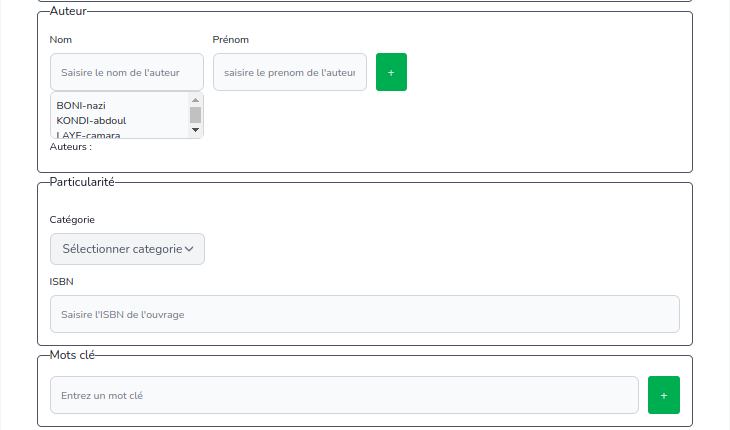
\includegraphics[scale=0.5]{images/APMelectro.png}.\\

\textbf{La section Résumé de l'ouvrage} qui contient le résumé de l'ouvrage.\\
\textbf{La section fichier pdf} qui nous permettra de charger nos fichier pdf à partir de notre machine et les insérer dans l'application.\\

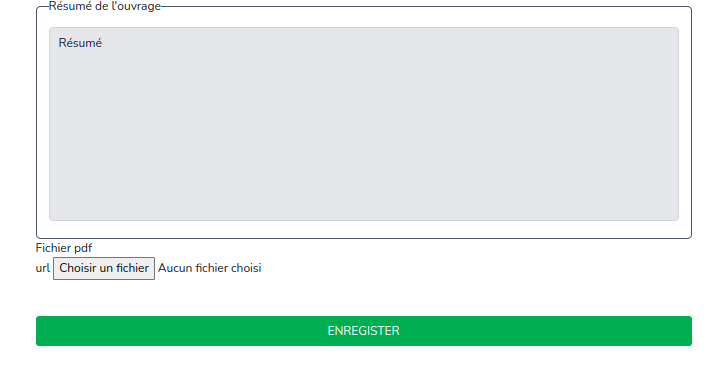
\includegraphics[scale=0.5]{images/ResumeFichier.png}.\\

\textbf{Après avoir entré toute les informations vous cliquez sur le boutons enregistrer afin de valider les informations entrée}.\\

\textbf{Pour ce qui est des options consulter, modifier et supprimer c'est pareil que celui de l'ouvrage physique}.\\

\newpage
\section{Accès à l'Emprunt}
Dans le barre de navigation cliquez sur le menu emprunt et vous serez dirigé vers le menu emprunt.\\

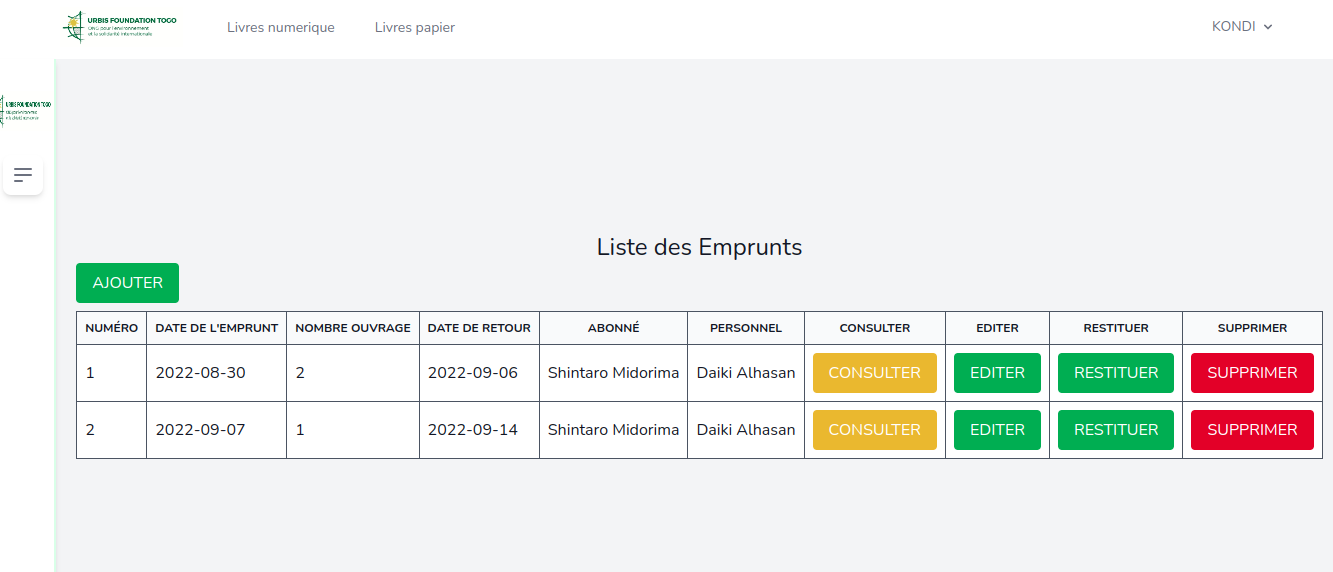
\includegraphics[scale=0.35]{images/Emprunt.png}.\\

Dans le menu Emprunt nous pouvons ajouter un emprunt, l'éditer, le consulter, le restituer ou le supprimer.

\begin{itemize}
\item[•]Etape 1: Ajoutons un Emprunt.
\end{itemize}

Pour ce faire nous allons cliquer sur le boutons \textbf{ajouter} 

\begin{itemize}
\item[•]Etape 2 : Remplissez les champs suivant avec des données conformes.
\end{itemize}

Comme champs à remplir nous avons :\\
\textbf{La section Abonne} qui contient le nom et prénom de l'abonne.\\

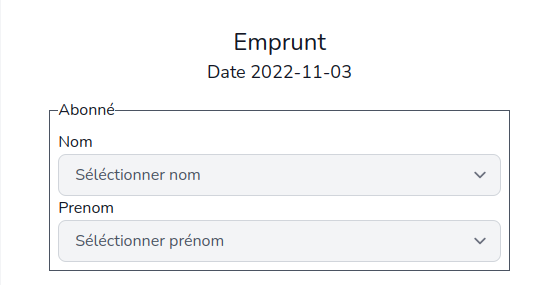
\includegraphics[scale=0.5]{images/Abonne.png}

\textbf{La section Ouvrage} qui contient la côte, le titre ainsi que l'état de l'ouvrage.\\

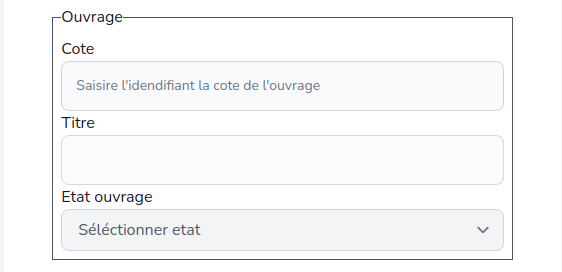
\includegraphics[scale=0.5]{images/EOuvrage.png}.\\

\textbf{La section Durée} qui contient la période à laquelle le livre a été prêté.\\
Pour cette partie lorsque vous finissez de remplir ce champs veuillez à cliquer sur le bouton ajouter vous verrez que l'emprunt à été ajouter et vous pouvez également ajouter un autre emprunt si l'abonné veux prendre par exemple deux ouvrages.\\

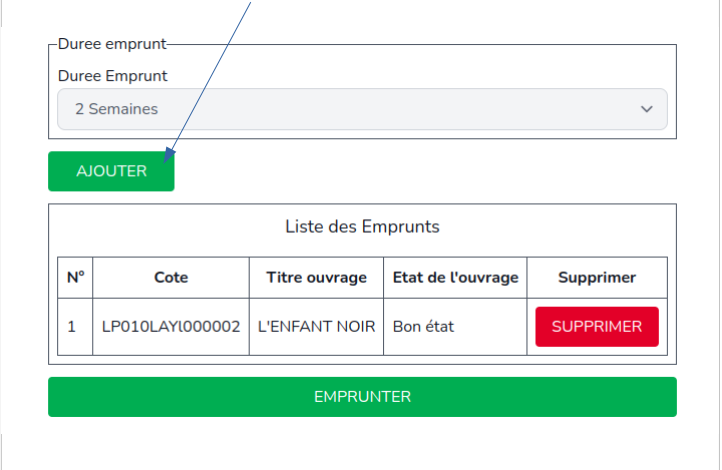
\includegraphics[scale=0.5]{images/EDureeAjout.png}.\\
Après l'avoir fait vous n'avez plus qu'à cliquez sur le bouton emprunter pour emprunter l'ouvrage.\\

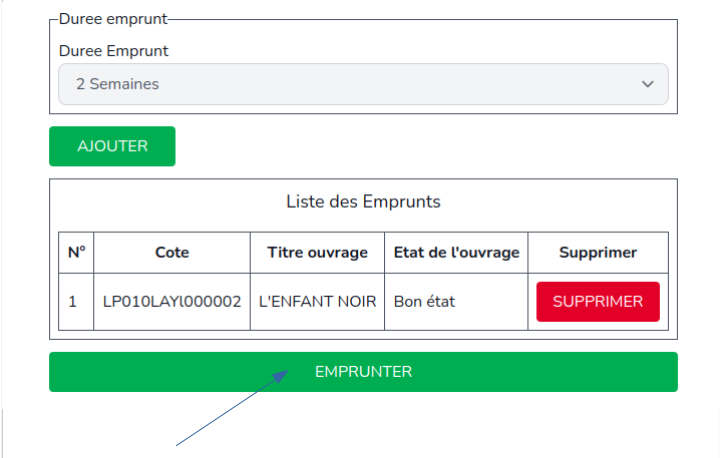
\includegraphics[scale=0.5]{images/EDureeEmprunt.png}.\\

\textbf{Lorsque vous décidez de consulter un emprunt en cours vous n'avez qu'à cliquez sur le bouton consulter}.\\

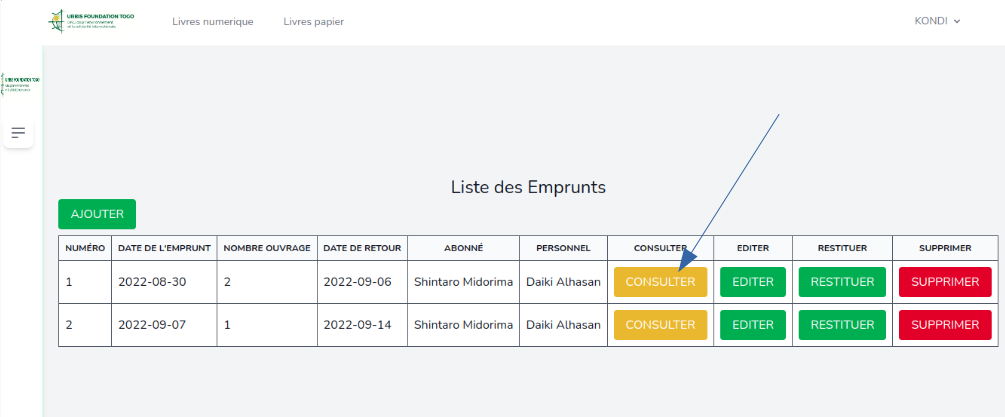
\includegraphics[scale=0.5]{images/ConsultEmprunt.png}.\\

Et comme résultat vous obtiendrai le nom et prénom de l'abonne ainsi que celui du personnel ayant effectué l'emprunt, le nombre d'ouvrage emprunté, la date d'emprunt et de retour.\\

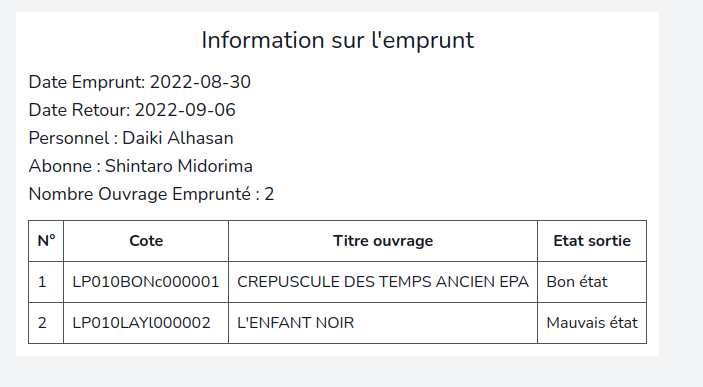
\includegraphics[scale=0.5]{images/ConsultationEmprunt.png}.\\

\newpage
\textbf{Dans le cas de la modification d'un Emprunt}.\\
Pour la modification de l'emprunt le plus important c'est le fait de prolonger l'emprunt de l'abonné.\\

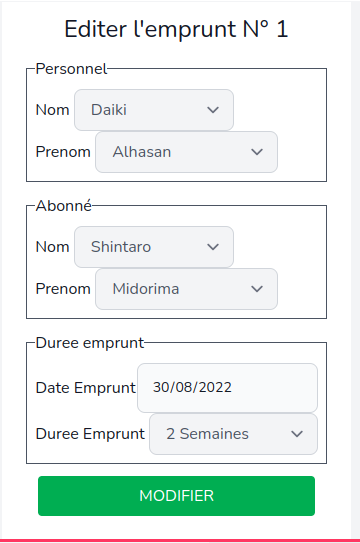
\includegraphics[scale=0.5]{images/EmpruntEdit.png}.\\

\textbf{Dans le cas de la restitution}.\\
Pour ce qui est de la restitution vous devez cliquer sur le bouton restitution.

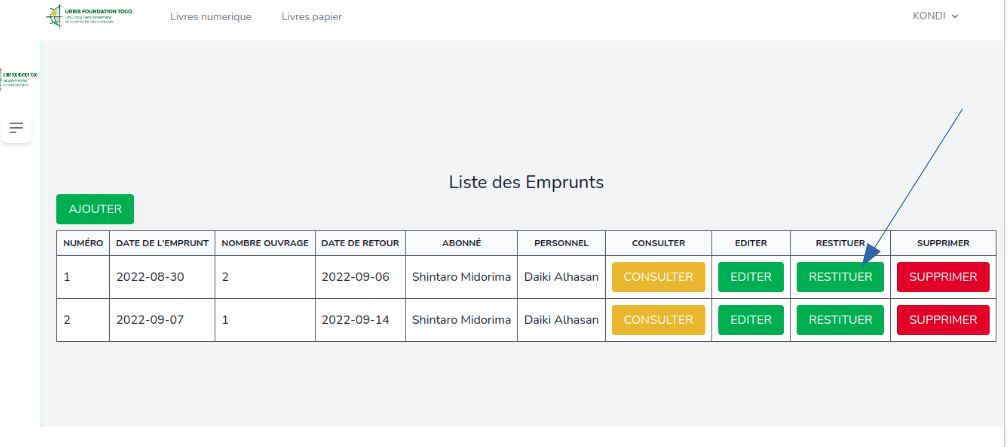
\includegraphics[scale=0.5]{images/RestitutionSectionner.png}.
\newpage
Après avoir sélectionnez le bouton restituer vous serez rediriger vers la page de restitution.\\

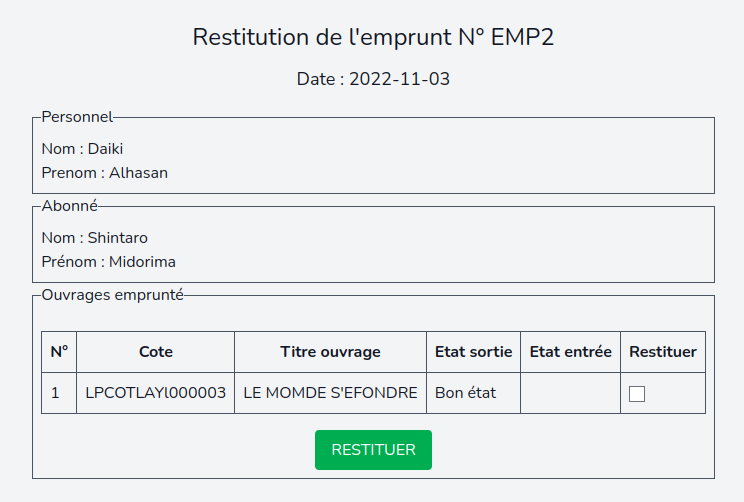
\includegraphics[scale=0.5]{images/Restitution.png}.\\

Pour effectuer la restitution vous devez cocher la case restitution afin de sélectionner l'état dans lequel le livre est restituer. Procédez comme suit :

\begin{itemize}
\item[•] Etape 1 : Cocher la case blanche au niveau de la colonne restituer.\\
\end{itemize}

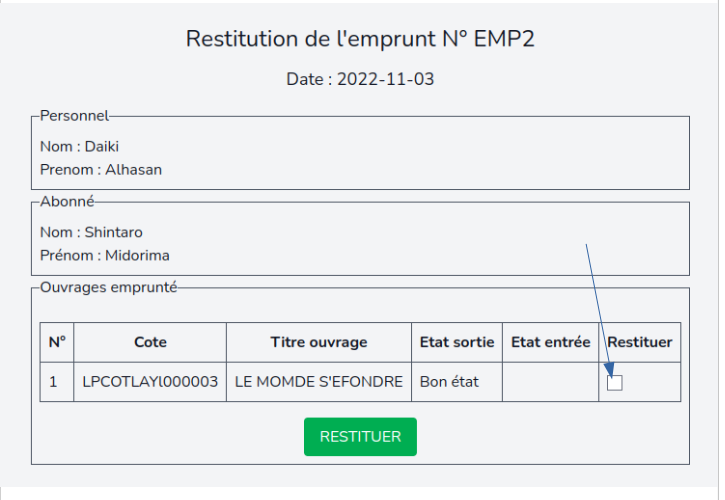
\includegraphics[scale=0.5]{images/Cocher.png}.\\

\newpage
Après avoir coché vous serez redirigé sur la page suivante : \\

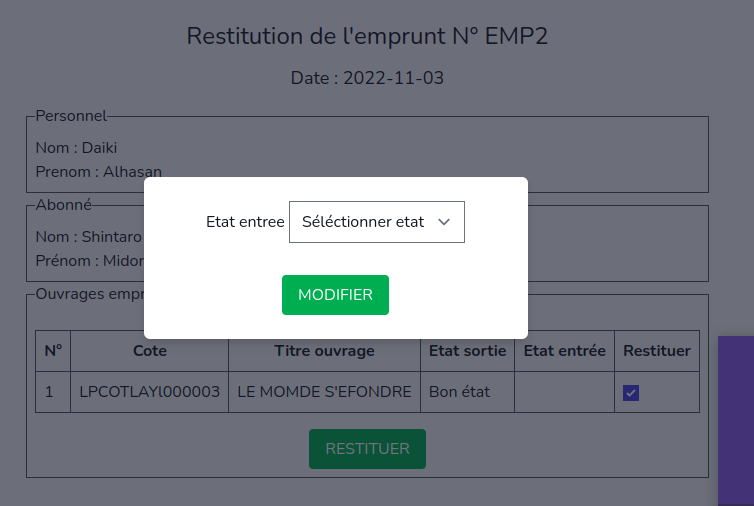
\includegraphics[scale=0.5]{images/SelectEtat.png}.\\


\begin{itemize}
\item[•] Etape 2 : Sélectionnez l'état du livre puis valider en cliquant sur modifier.
\end{itemize}

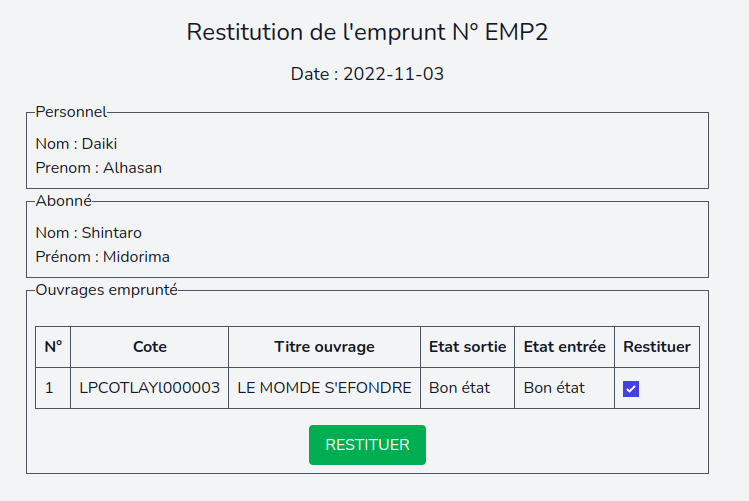
\includegraphics[scale=0.5]{images/Restitutionbouton.png}.\\

\newpage
\begin{itemize}
\item[•] Etape 3 : Cliquer sur restituer pour restituer l'ouvrage.\\
\end{itemize}

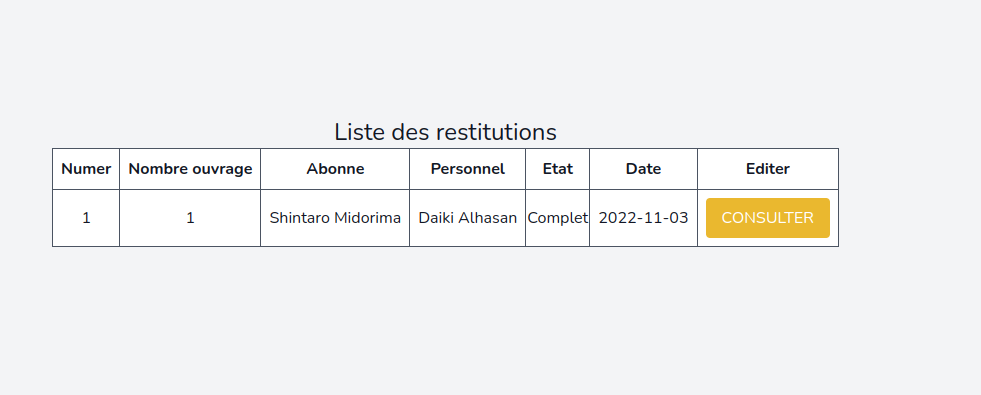
\includegraphics[scale=0.5]{images/ListeDesRestitutions.png}

\section{Accès à la restitution}
Dans le barre de navigation cliquez sur le menu restitution et vous serez dirigé vers le menu restitution.\\

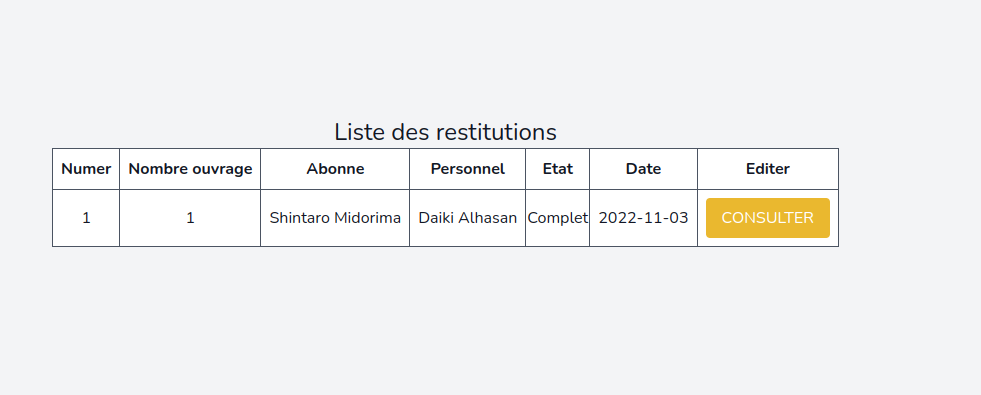
\includegraphics[scale=0.5]{images/ListeDesRestitutions.png}.

Ici comme option vous pouvez consulter toute les informations relative à la restitution.\\
\textbf{Accédons à l'option consulter de la restitution}.\\

Comme information nous avons le nom et prénom de l'abonné ainsi que tu personnel ainsi que tous les détails relative à l'emprunt de l'ouvrage notamment la côte, le titre, l'état de sorti et de retour de l'ouvrage et si l'ouvrage est totalement restituer ou partiellement.

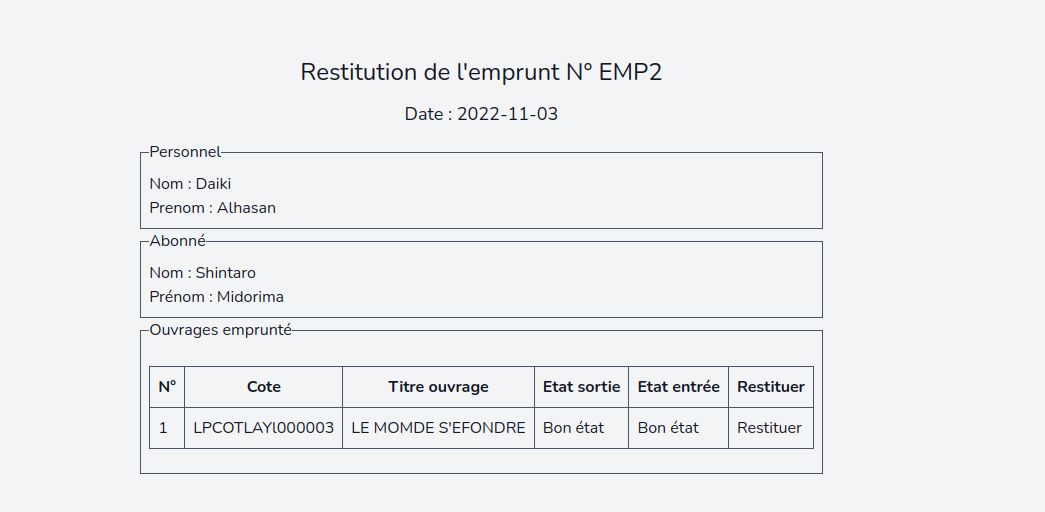
\includegraphics[scale=0.5]{images/showRestitution.png}













\newpage
\section{Gestion des utilisateurs}
Le menu gestion des utilisateurs comme vous pouvez facilement le deviné est un menu qui
nous permet de gérer les abonnés, leurs abonnements et le personnel. 
Pour accéder à ce menu, cliquez sur le bouton sur le quelle trois (3) traits on été marqué. 
Il se trouve à gauche de l'écran dans une barre vertical (barre latérale). \\

\begin{center}
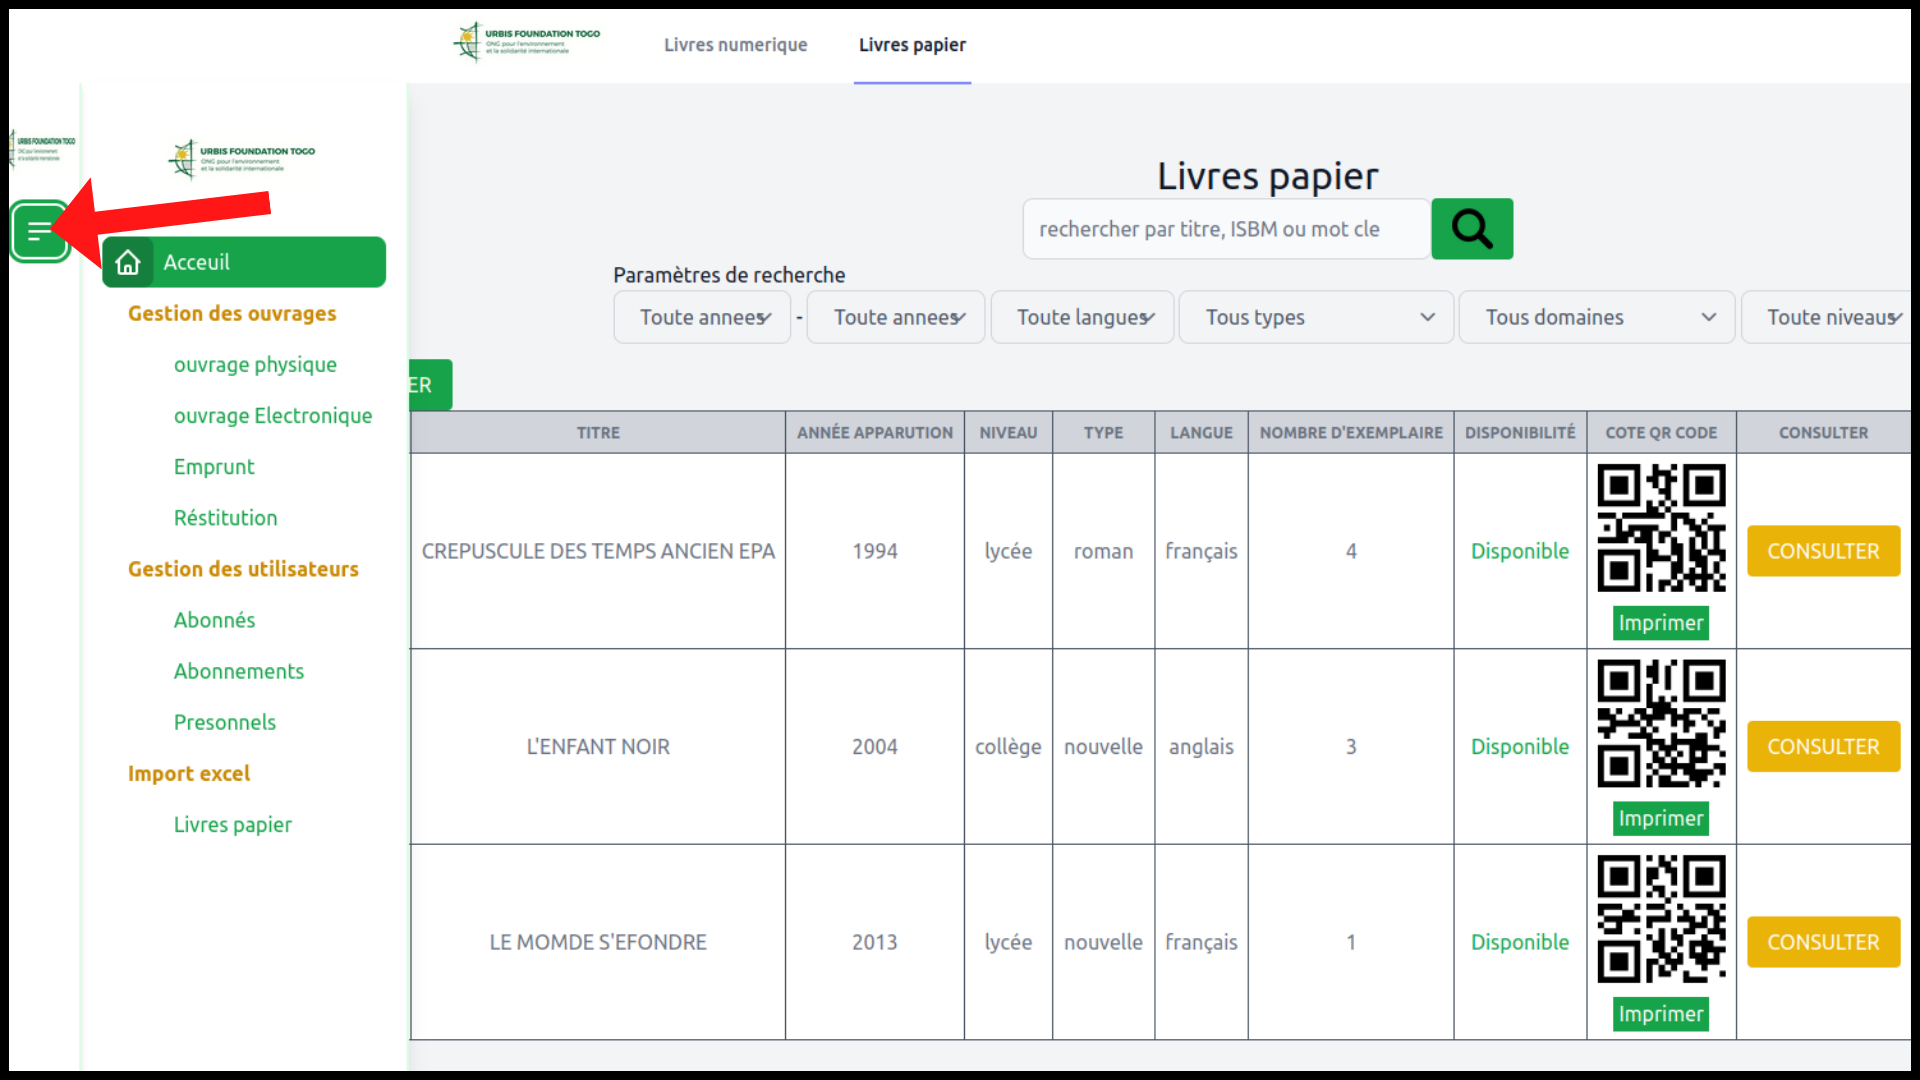
\includegraphics[scale=0.5]{img/sidebar.png}
\end{center}

\begin{center}
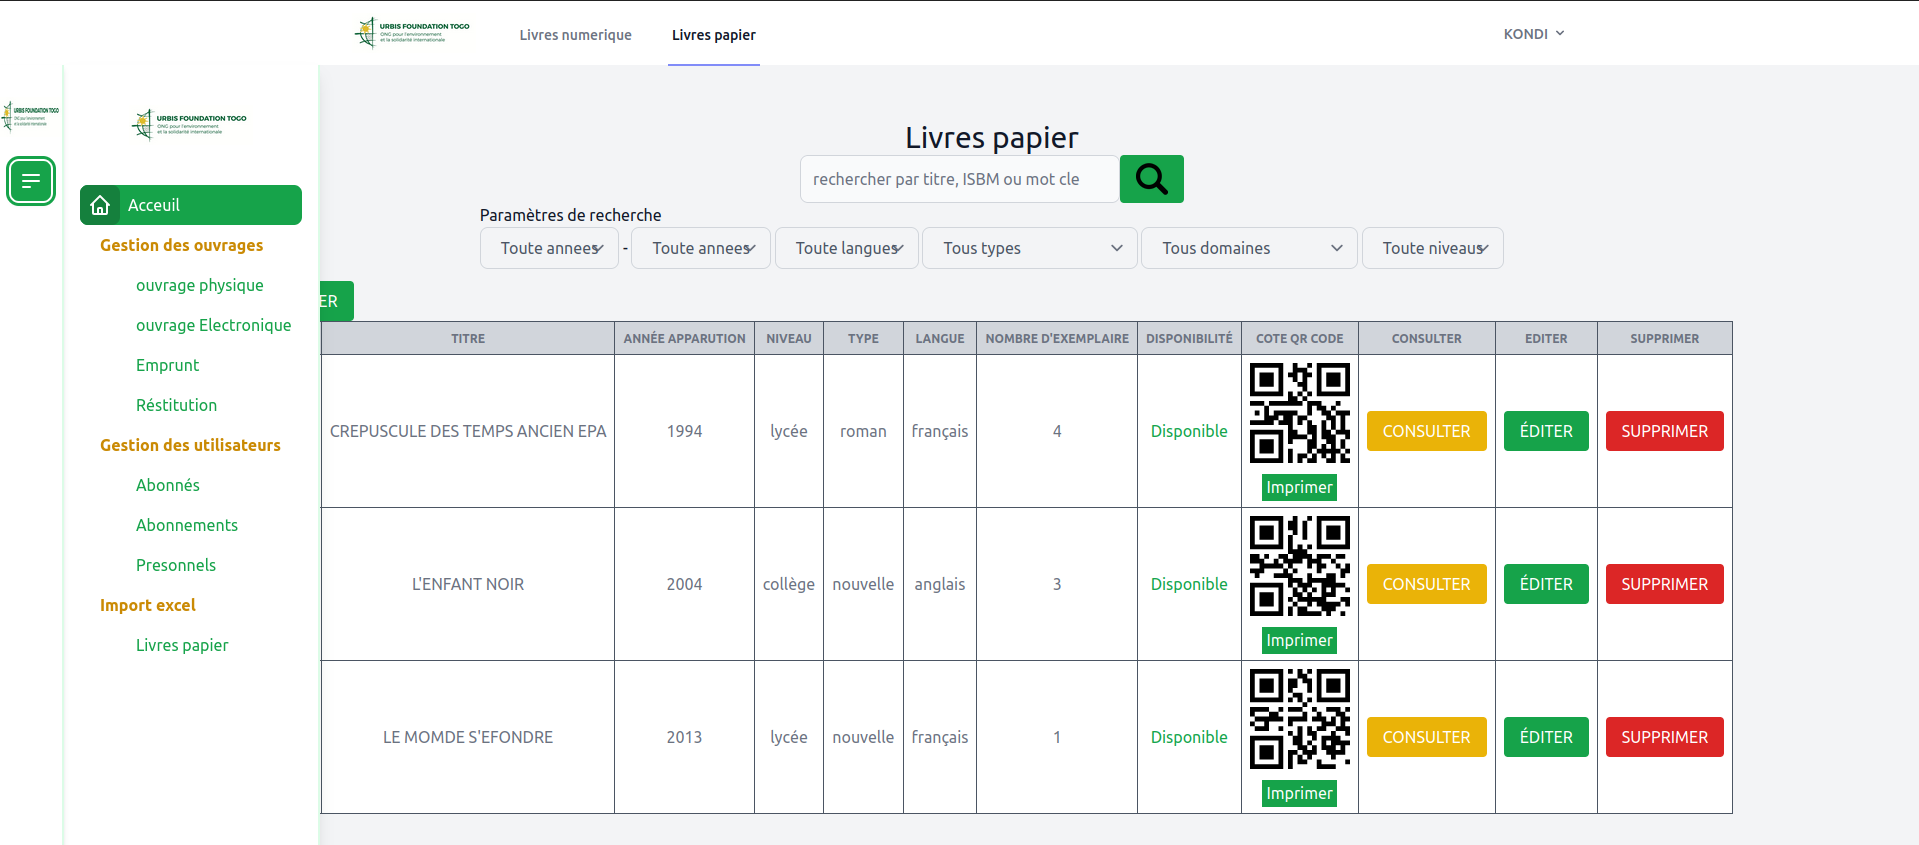
\includegraphics[scale=0.5]{img/gestion_utilisateurs.png}
\end{center}

Une fois que vous avez cliqué sur ce bouton, vous remarquerez qu'un quart (1/4) de page 
sortir de la gauche de l'écran. Rendez vous maintenant au menu \textbf{Gestion des
utilisateurs} écrit en jaune. Vous y verrez trois sous menus :
\begin{itemize}
\item[•] Abonnés
\item[•] Abonnements
\item[•] Personnels
\end{itemize}

\newpage
\subsubsection{Sous menu \textbf{Abonnés}}
Cliquez sur \textbf{Abonnés}.
\begin{center}
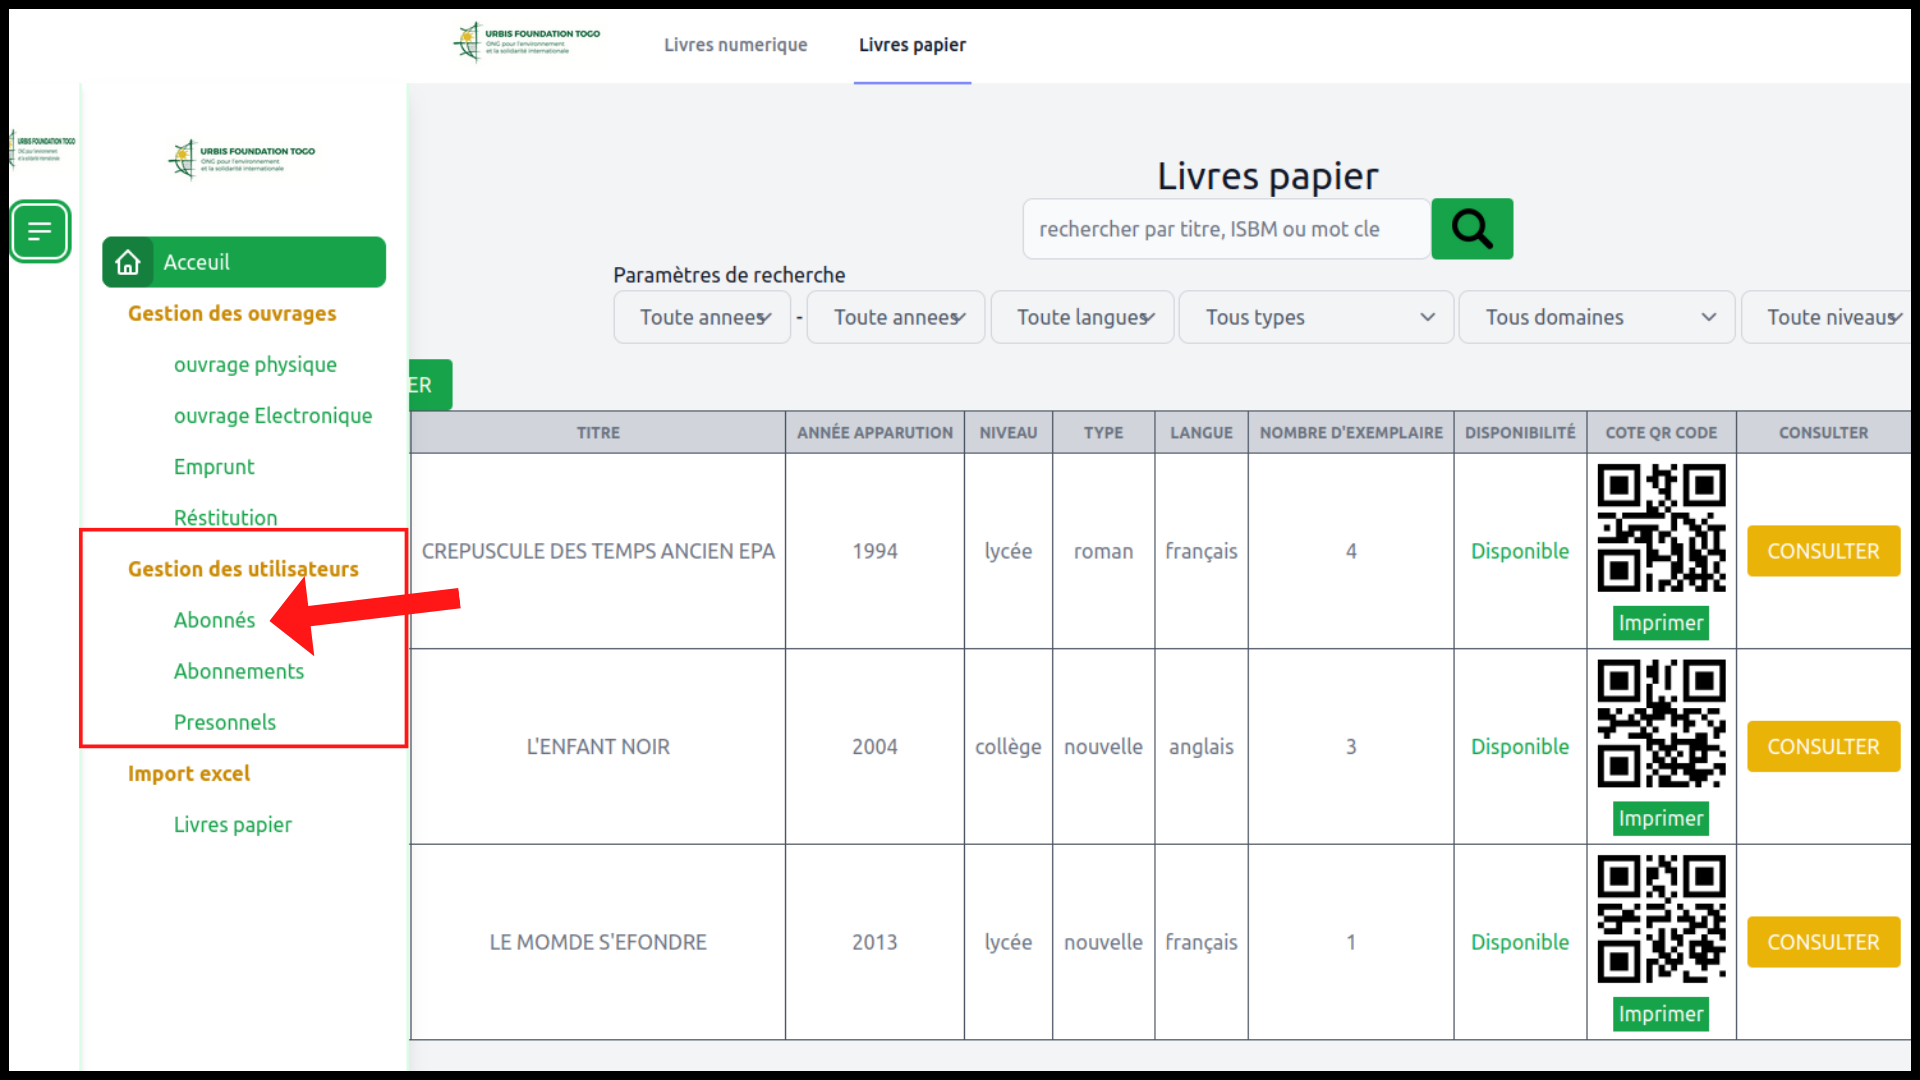
\includegraphics[scale=0.5]{img/abonne_menu.png}
\end{center}
vous verrez cette page s'afficher.\\
\begin{center}
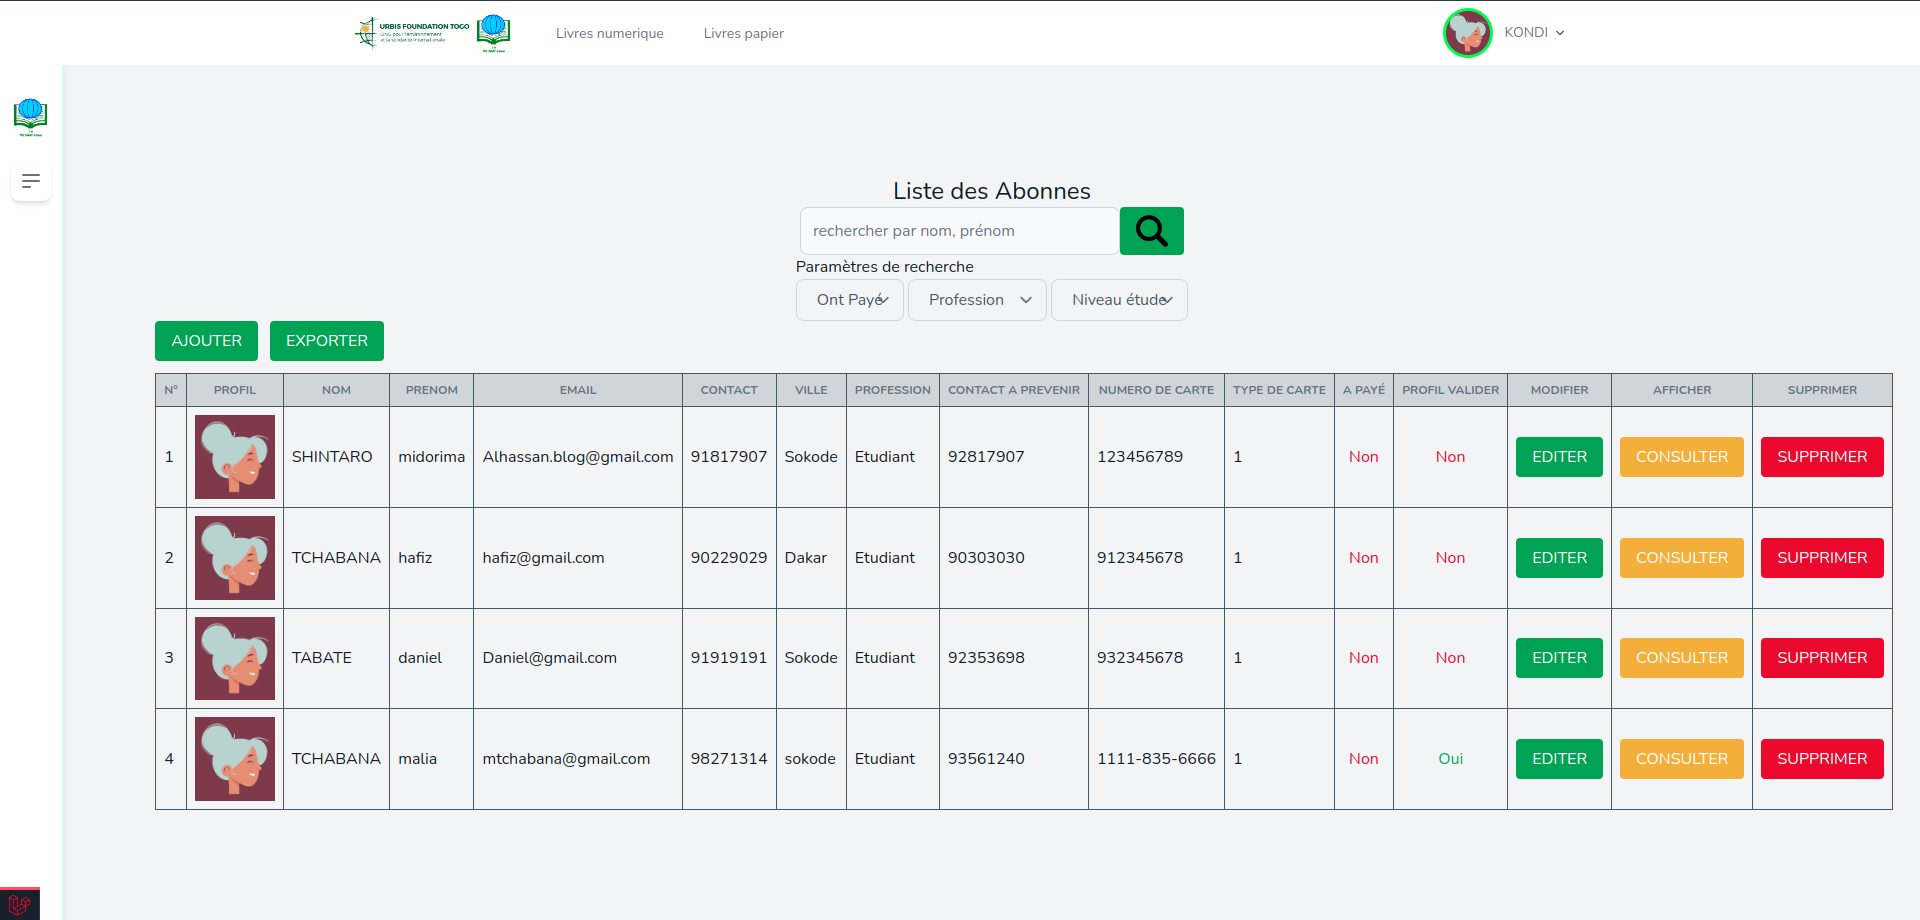
\includegraphics[scale=0.3]{img/abonnes_liste.png}
\end{center}
Cette pages contient :
\begin{itemize}
\item Une barre de recherche avec quelque paramètres de recherche.
\item Un bouton \textbf{AJOUTER}
\item Un bouton \textbf{Exporter}.
\item Et la liste des abonnés afficher dans un tableau. Pour chaque abonnés vous aurez trois boutons : 
\textbf{CONSULTER}, \textbf{ÉDITER}, \textbf{SUPPRIMER}.\\
\end{itemize}
Explication de chaque partie cité plus haut : 
\begin{itemize}
\item La barre de recherche permet de filtrez la liste des abonnées. On peut ainsi filtrer 
les abonnées par profession, niveau d'étude ou par abonnement.\\

\begin{center}
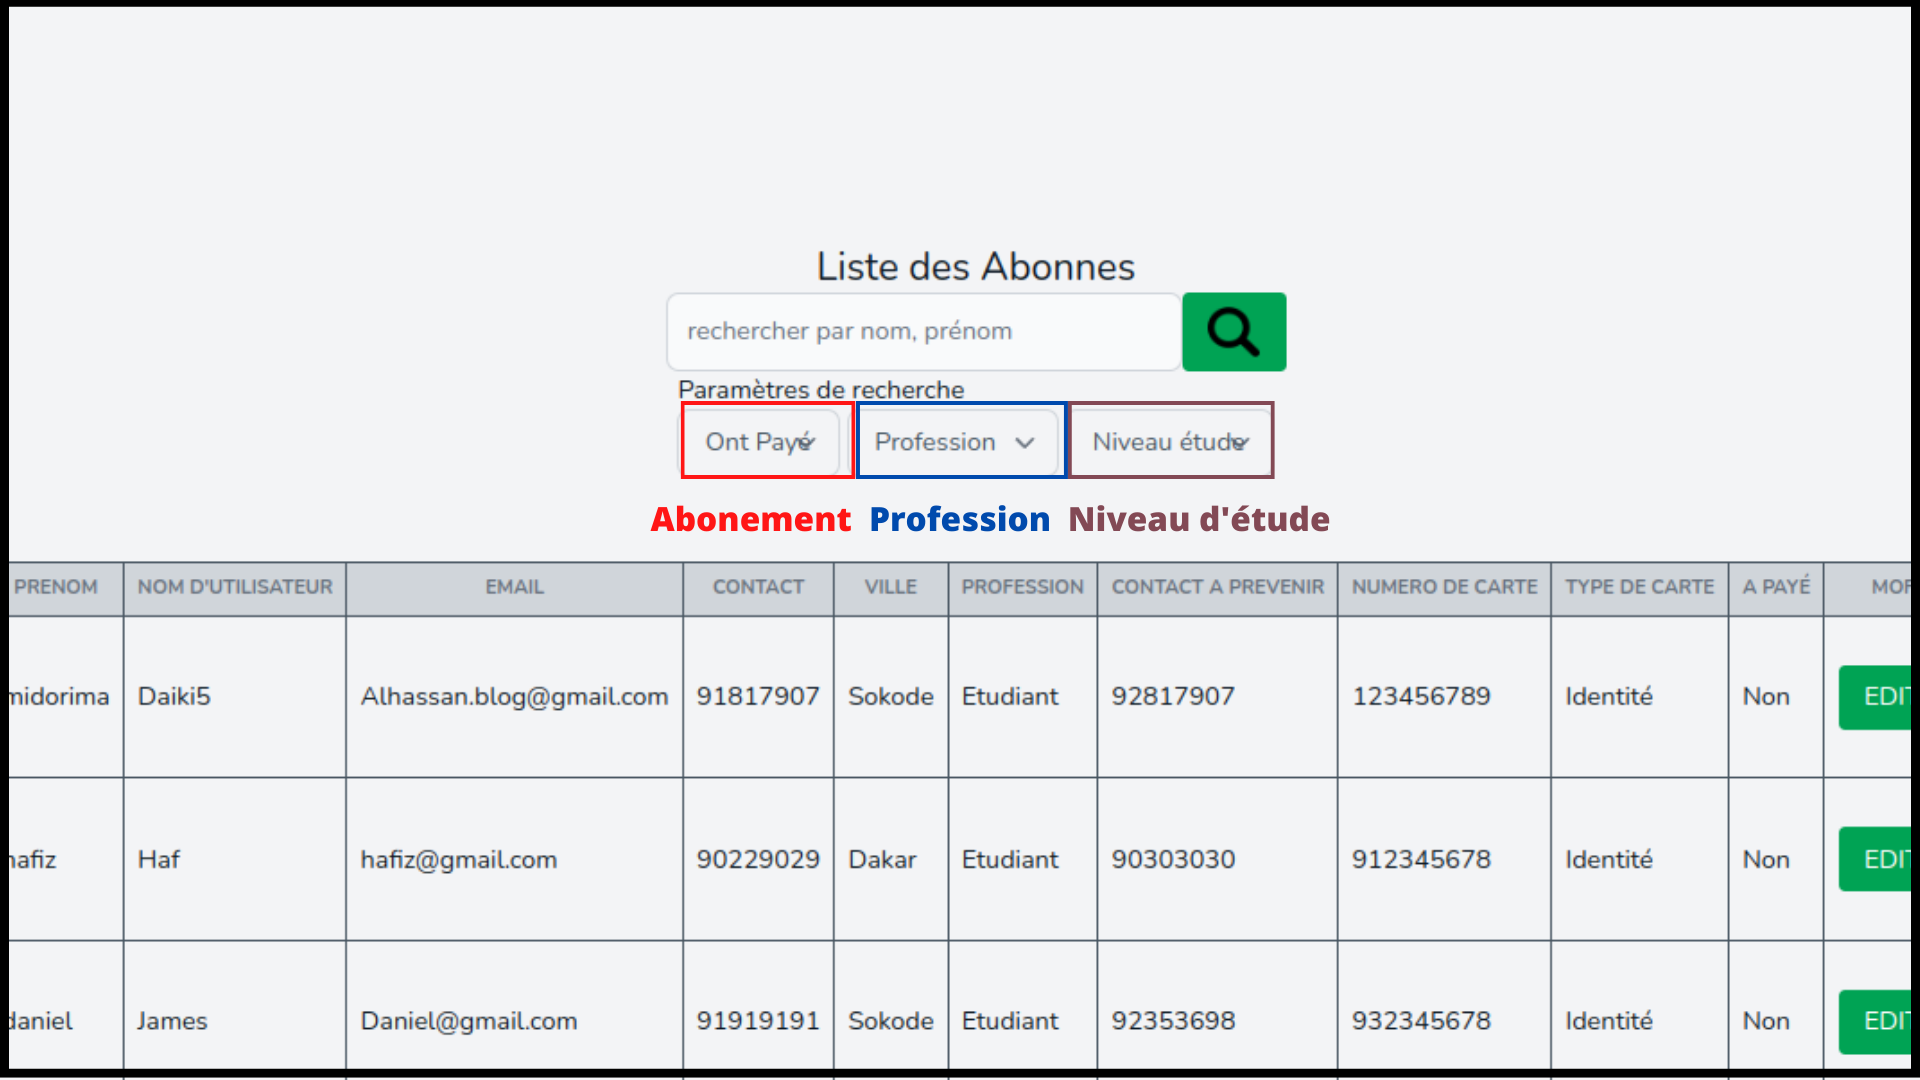
\includegraphics[scale=0.3]{img/abonne_search.png}
\end{center}

Pour filtrez cliquer sur le bouton rechercher.

\begin{center}
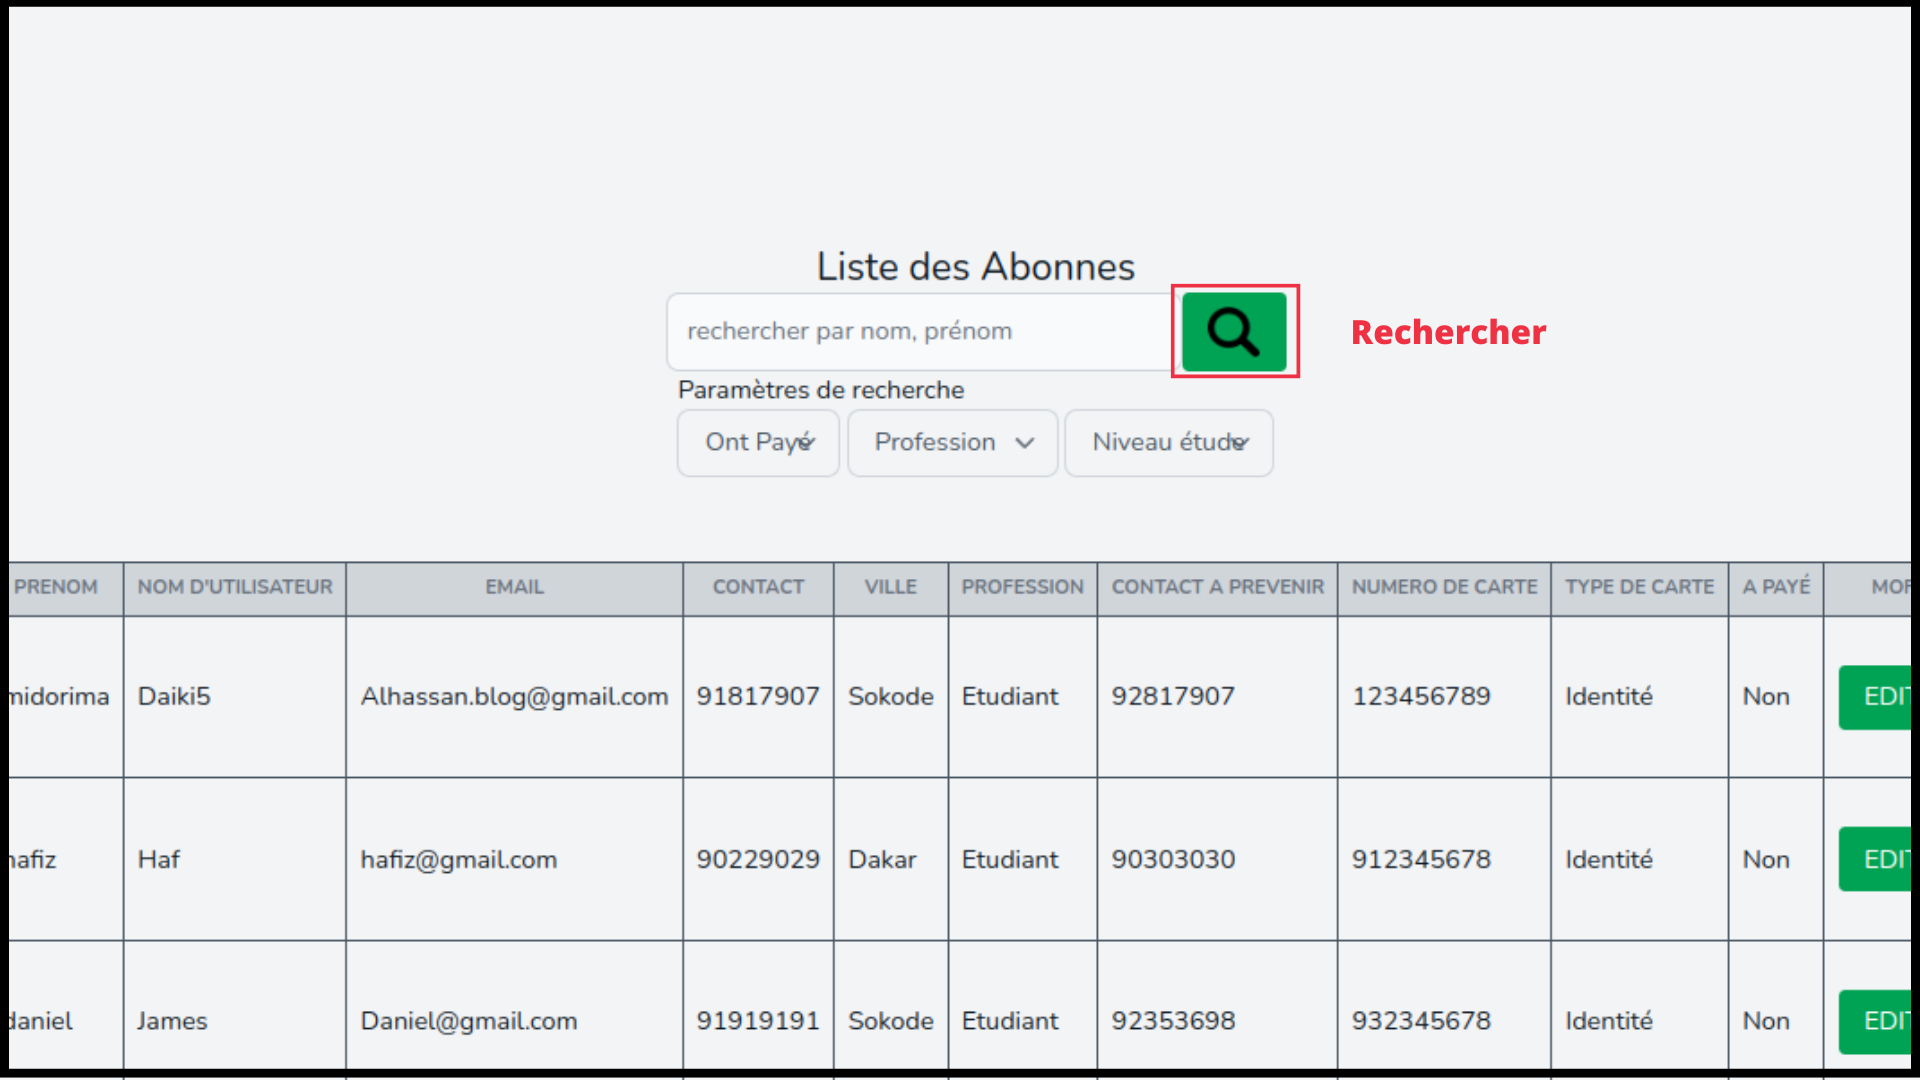
\includegraphics[scale=0.3]{img/abonne_search_button.png}
\end{center}

\item[•] Bouton \textbf{AJOUTER} : \\
Il permet d'enregistrer un nouvelle abonné.
\begin{center}
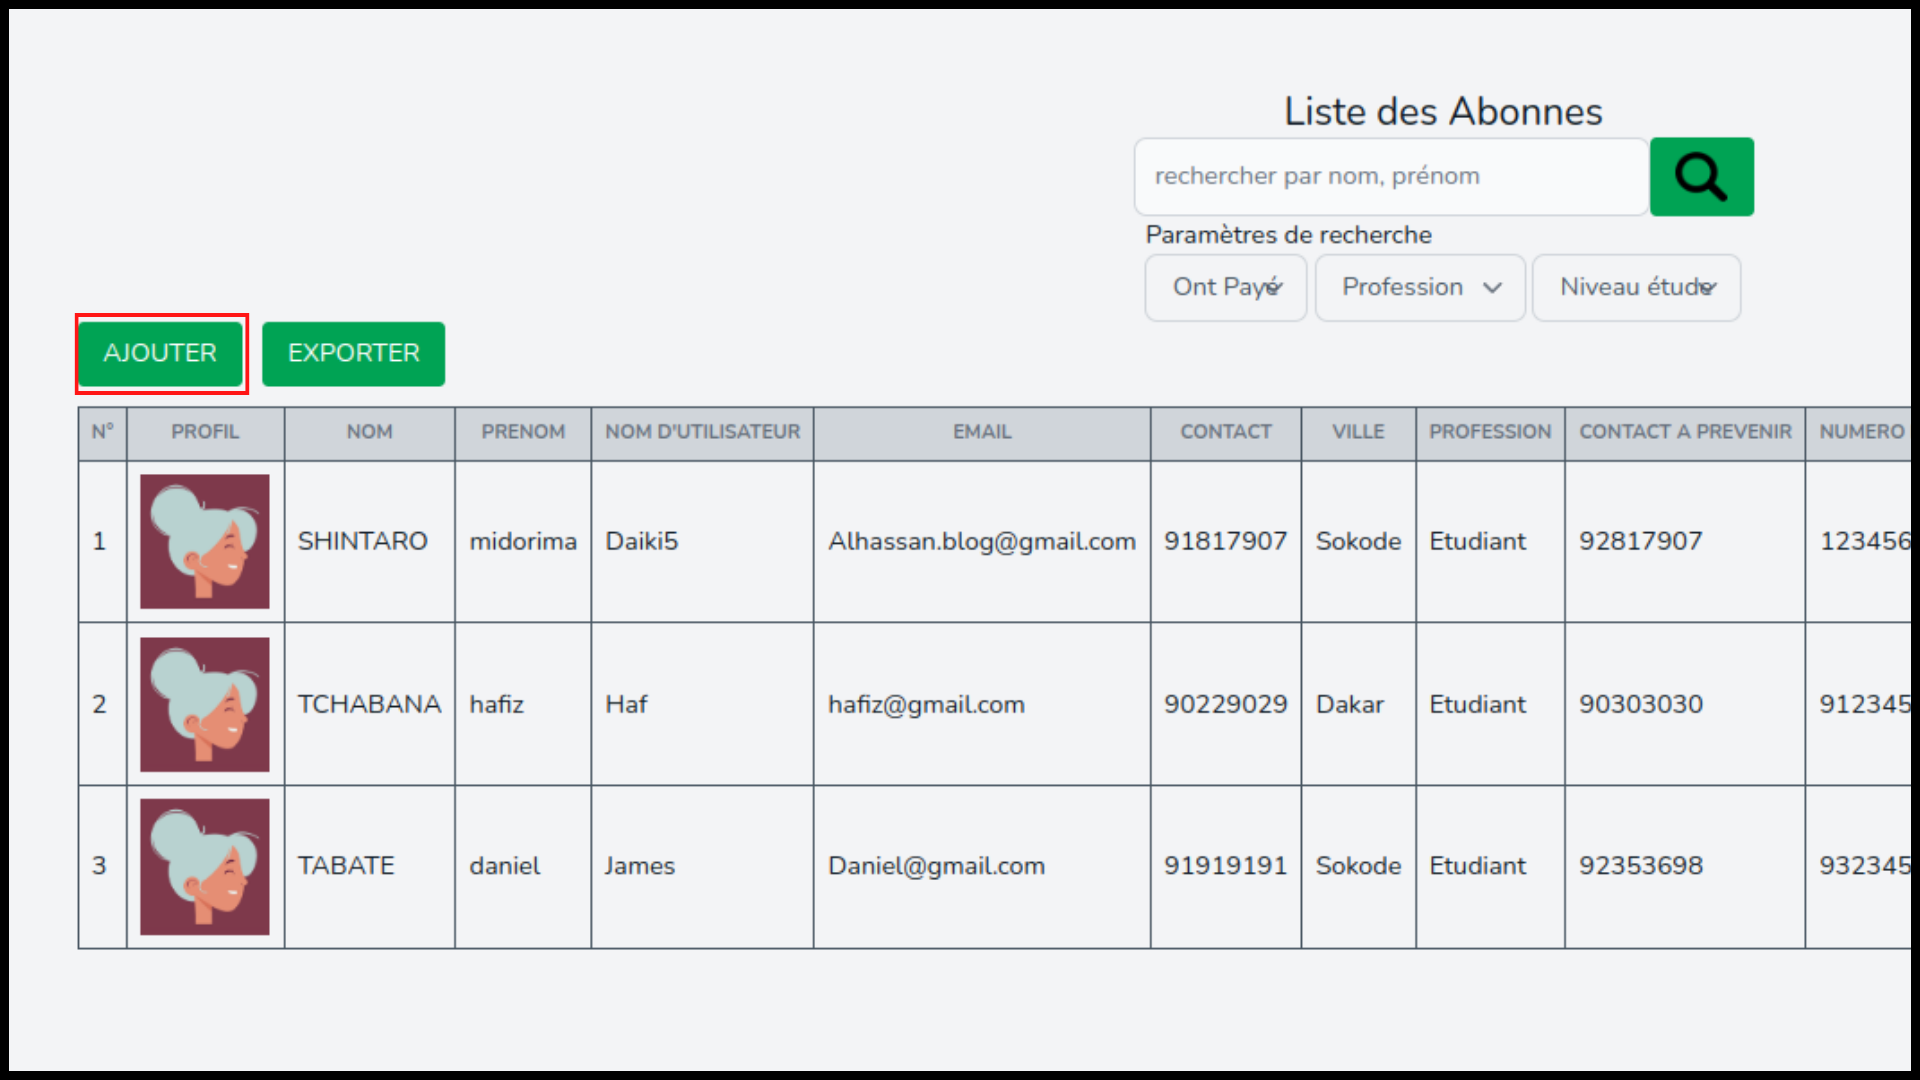
\includegraphics[scale=0.3]{img/abonne_create.png}
\end{center}
Cliquer dessus. C'est fait ? Vous verrez
une nouvelle page apparaître. 
\begin{center}
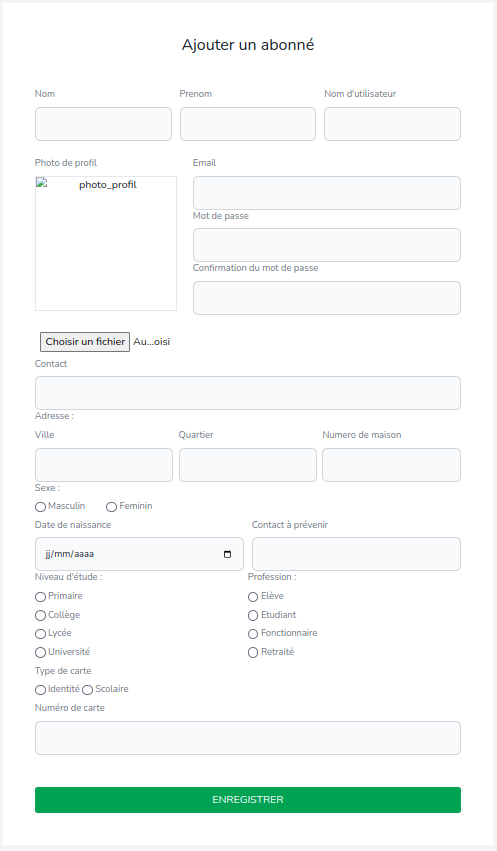
\includegraphics[scale=0.8]{img/abonne_save.png}
\end{center}
\textbf{NB:} 
\begin{itemize}
\item[-] Tous les champs sauf les champs ceux suivis de la mention optionnel(écrit en vers) sont obligatoire pour enregistrer un abonné.
\item[-] Pour indiquer \textbf{Oui} sur le champs profils validé, il vous faut vous même demander à l'abonné,
une pièce prouvant la validité des informations renseigné dans le formulaire.
\end{itemize}

Renseignez les informations relatif à l'abonné puis cliquer sur le
bouton enregistrer (il se trouve tout en bas).On est de retour sur la liste des abonnés avec cette fois ci
un abonné en plus.\\
\begin{center}
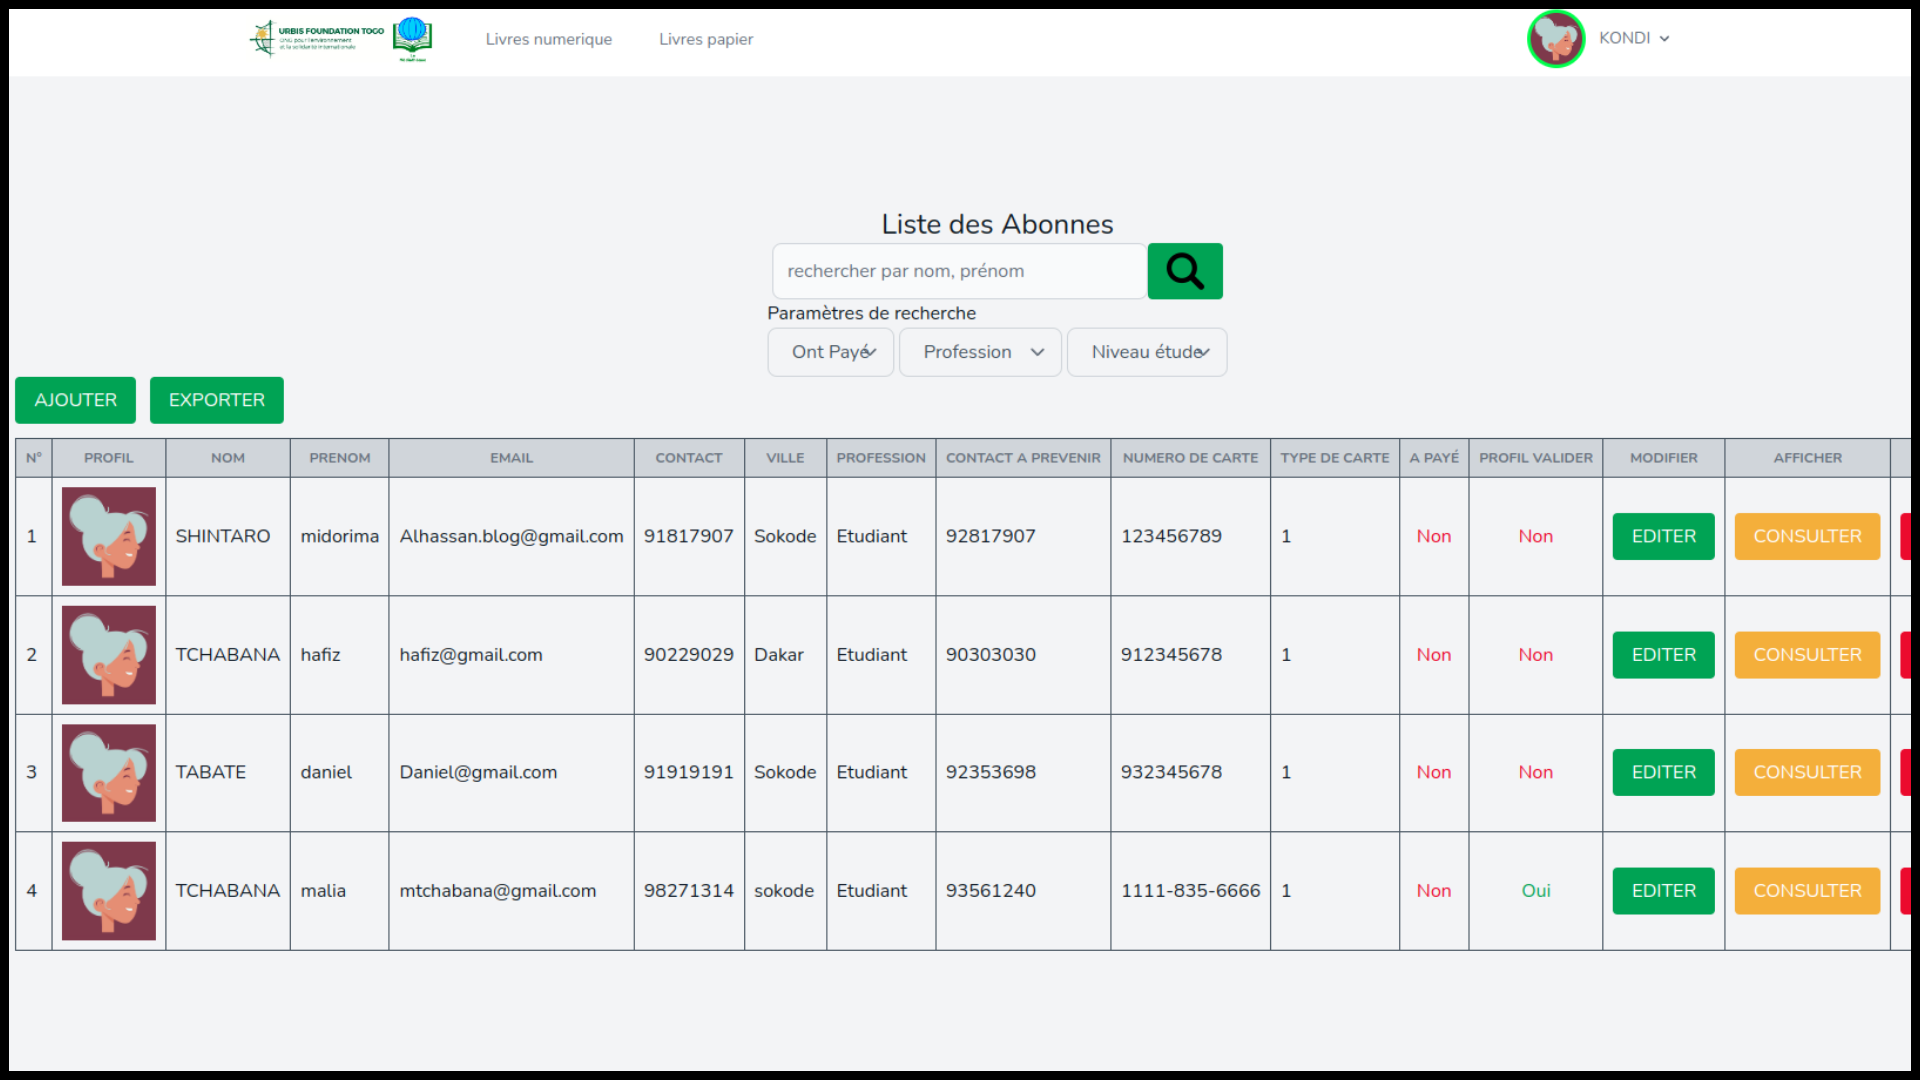
\includegraphics[scale=0.33]{img/abonnes_liste2.png}
\end{center}

\item[•] Bouton \textbf{EDITER} : \\
Il permet de modifier une information sur l'abonné ciblé. Nous souhaitons modifier les informations de
l'abonné malia.
\begin{center}
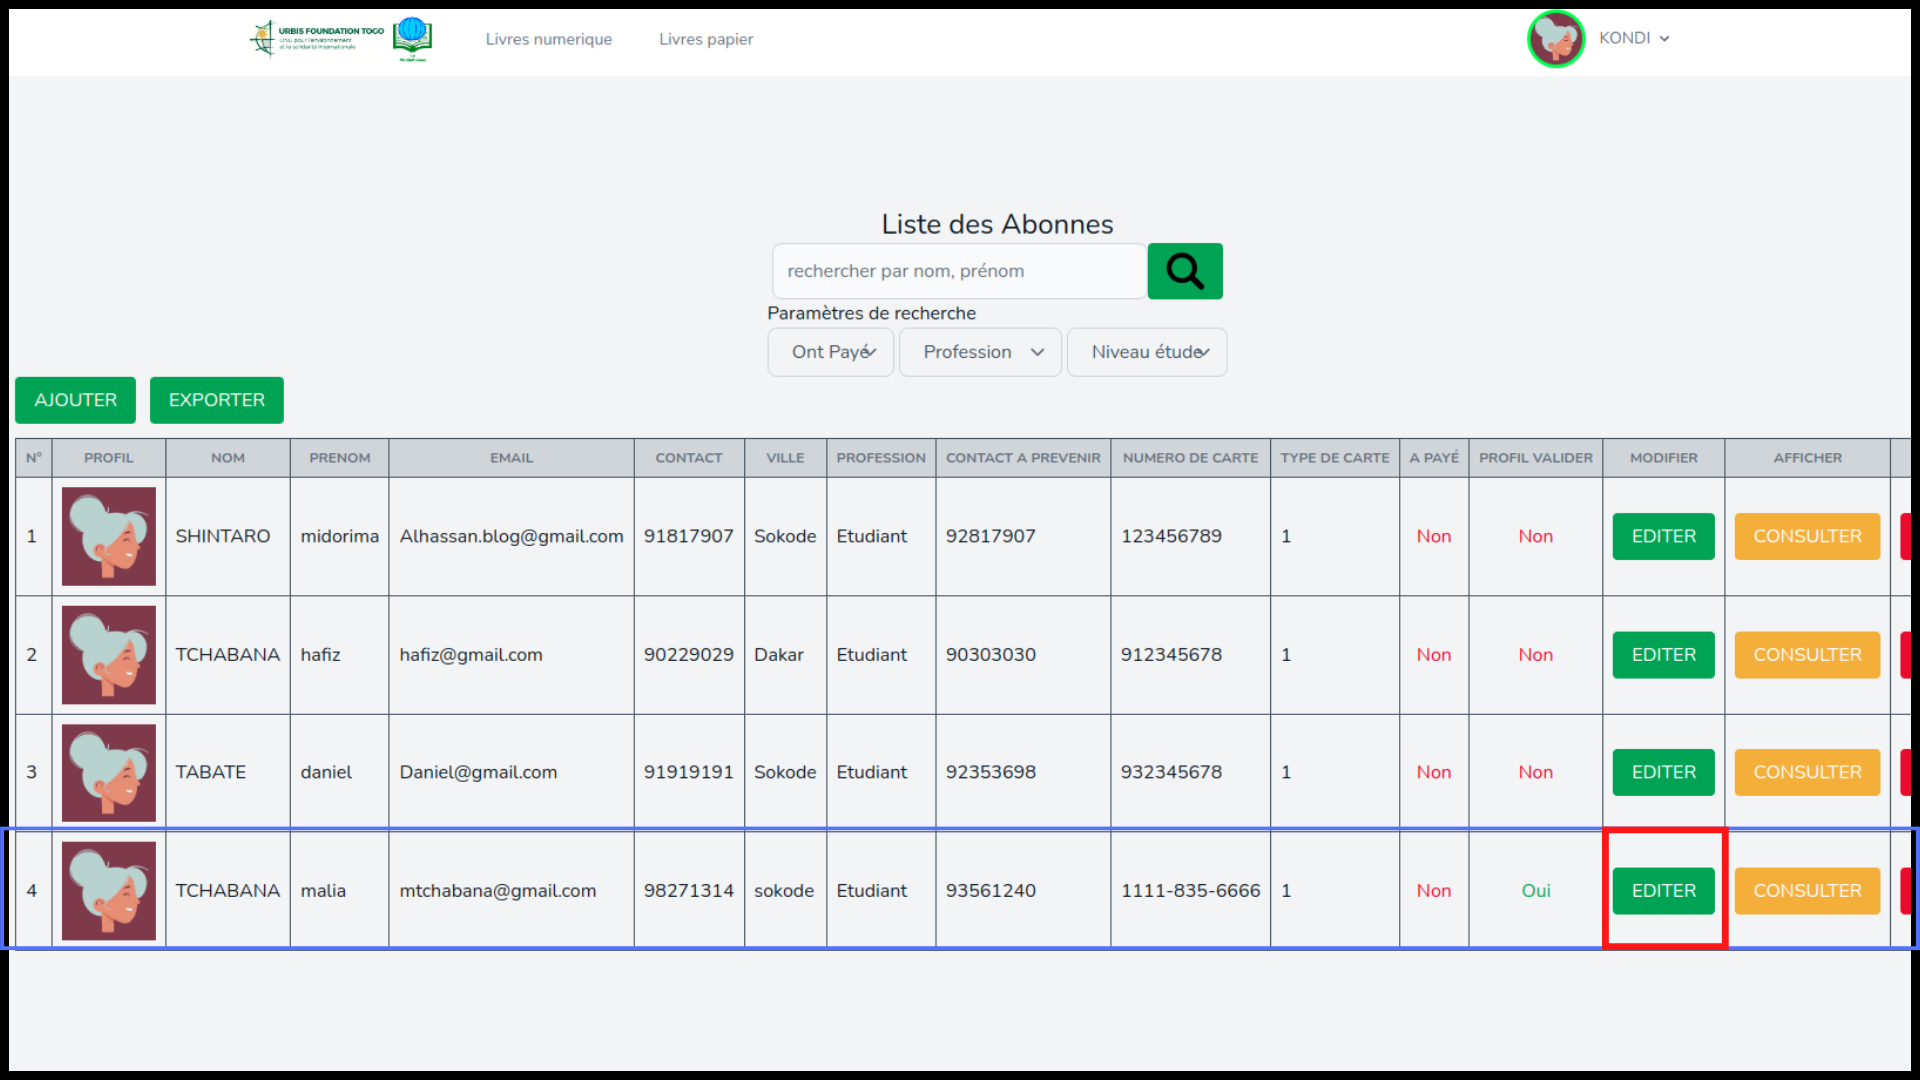
\includegraphics[scale=0.33]{img/abonne_edit_btn.png}
\end{center}
Cliquer dessus. Vous verrez s'afficher quelque chose de similaire.
\begin{center}
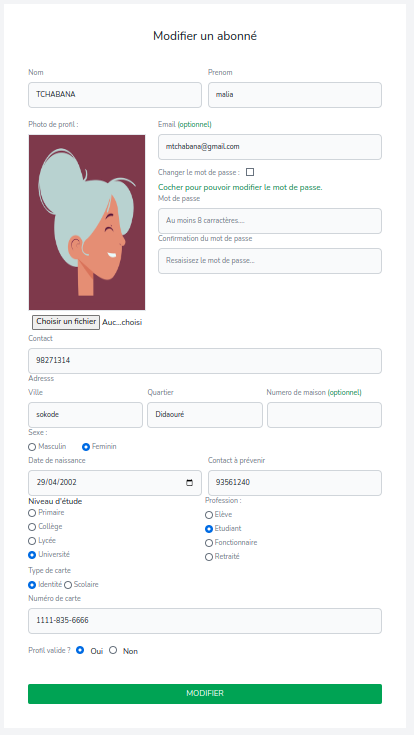
\includegraphics[scale=0.8]{img/abonne_edit.png}
\end{center}
Si nous voulons par exemple changer le numéro de la personne à prévenir pour quelconque 
raison, nous pouvons le ressaisir comme ceci et cliquer sur le bouton modifier.
\begin{center}
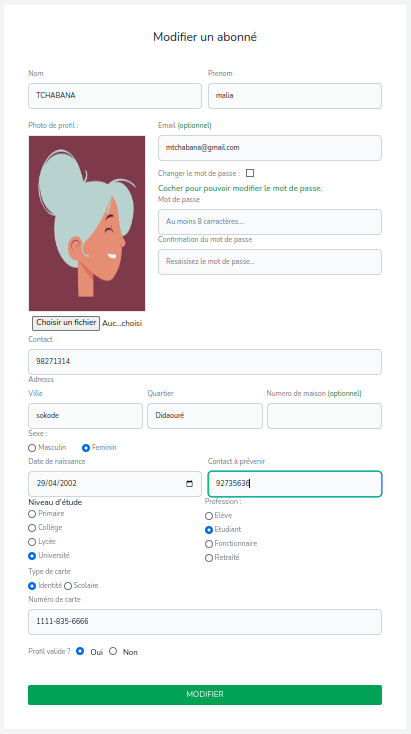
\includegraphics[scale=0.8]{img/abonne_edit_2.png}
\end{center}
Voici le résultat.\\
\begin{center}
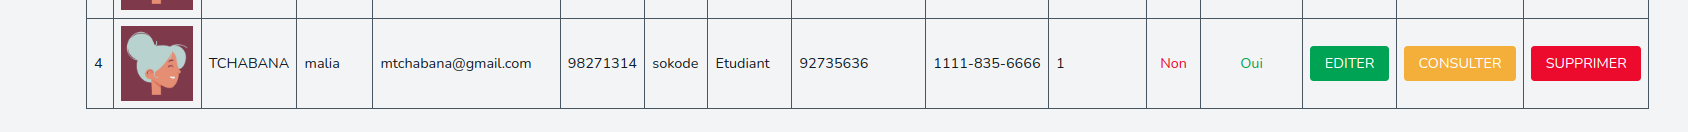
\includegraphics[scale=0.3]{img/abonne_edit_confirm.png}
\end{center}
Vous remarquerez que le contact a été modifier de \textbf{93561240} il est devenue \textbf{92735636}.

\item[•] Bouton \textbf{CONSULTER} : \\
Il permet d'accéder à toute les informations de l'abonné ciblé. Nous souhaitons afficher toute les informations 
de l'abonné malia.
\begin{center}
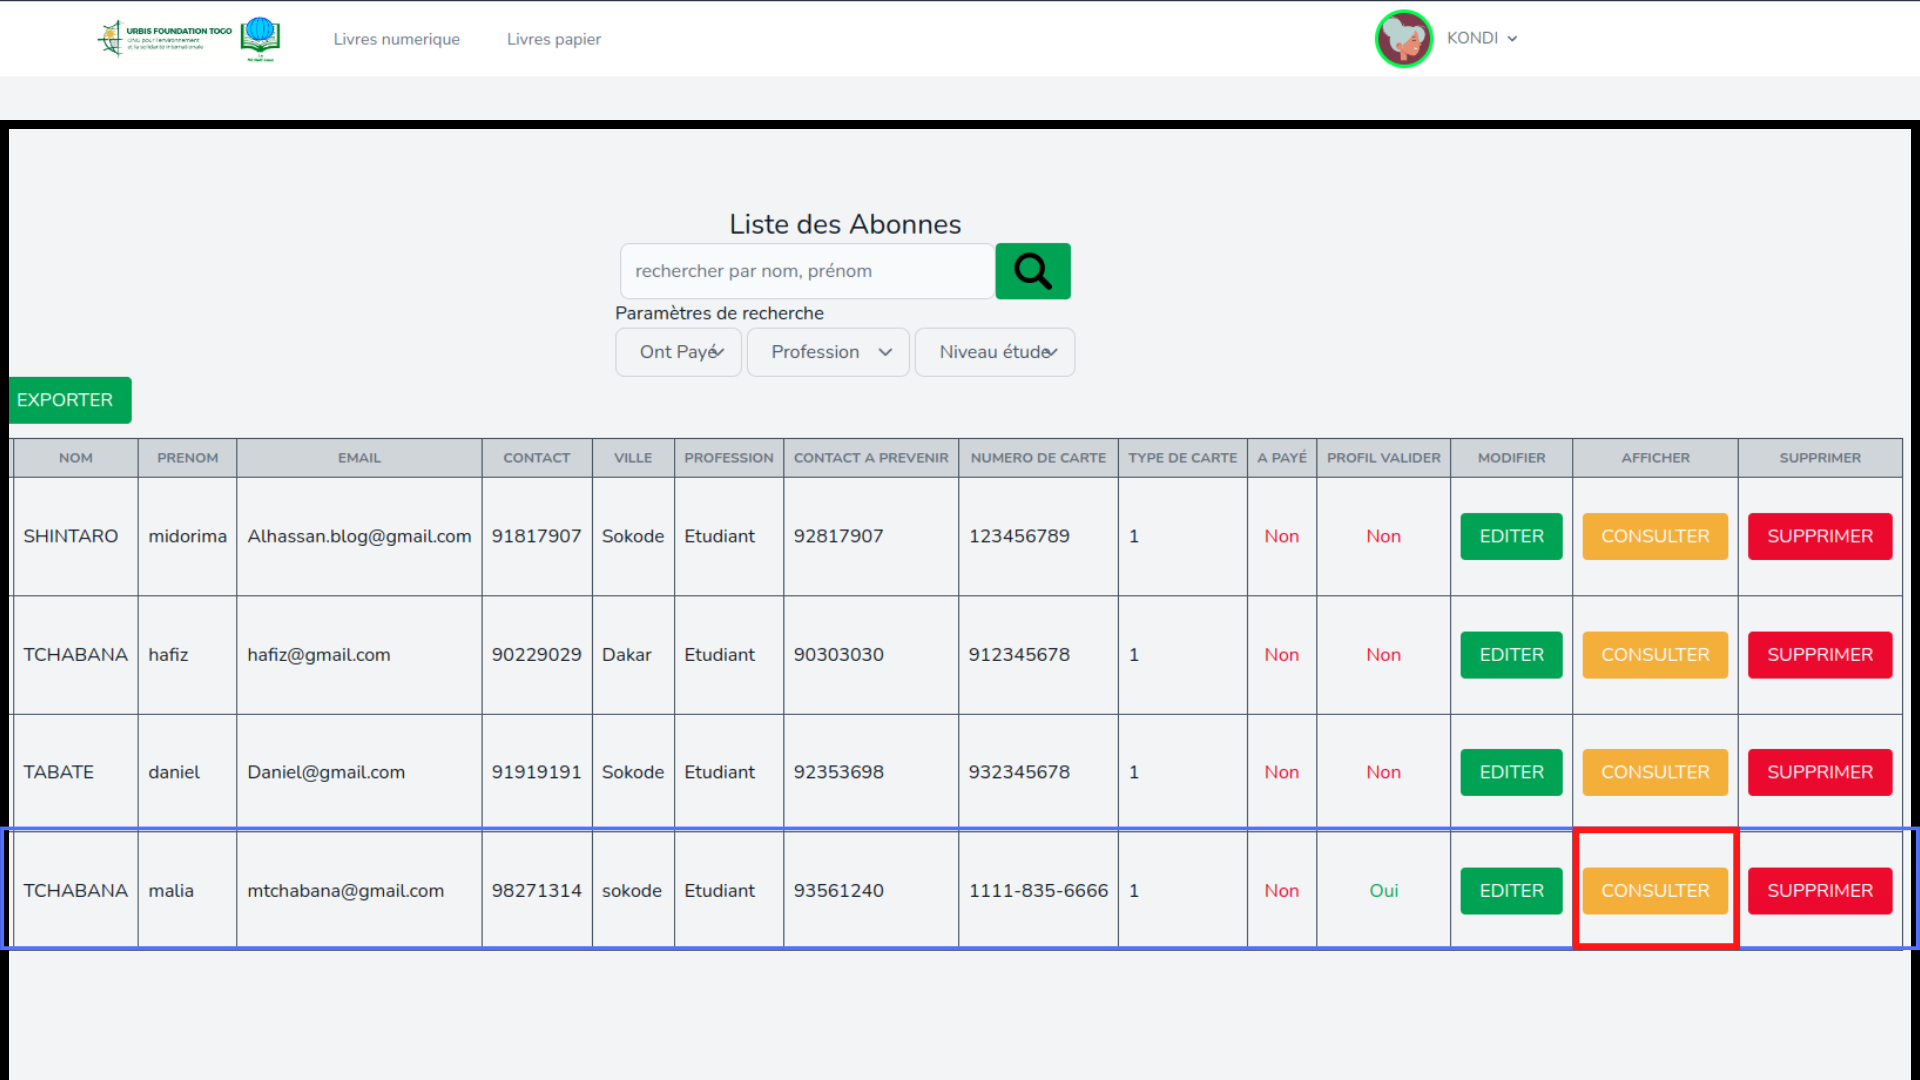
\includegraphics[scale=0.33]{img/abonne_show_btn.png}
\end{center}
Cliquer dessus. Vous verrez s'afficher quelque chose de similaire.
\begin{center}
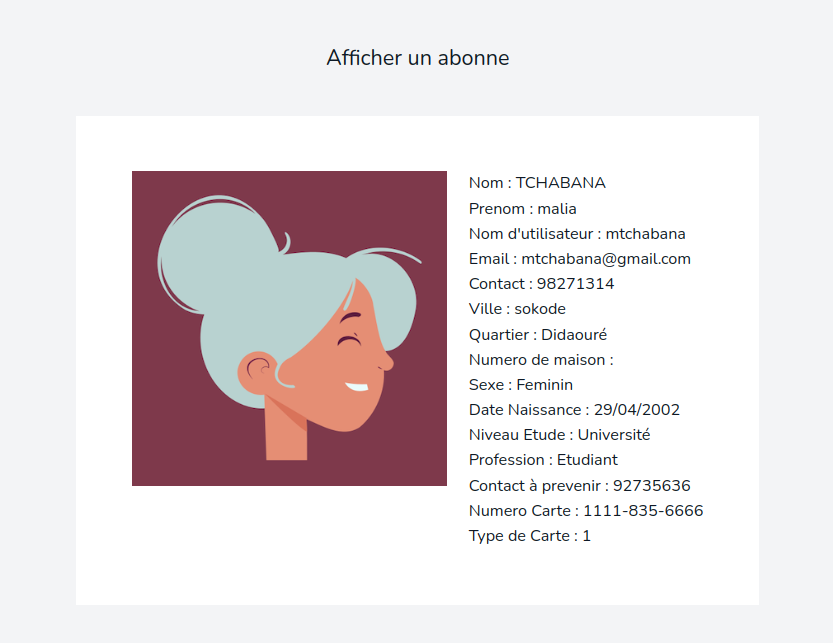
\includegraphics[scale=0.5]{img/abonne_show.png}
\end{center}

\item[•] Bouton \textbf{SUPPRIMER} : \\
Il permet de supprimer l'abonné ciblé. Cliquer dessus. 
\begin{center}
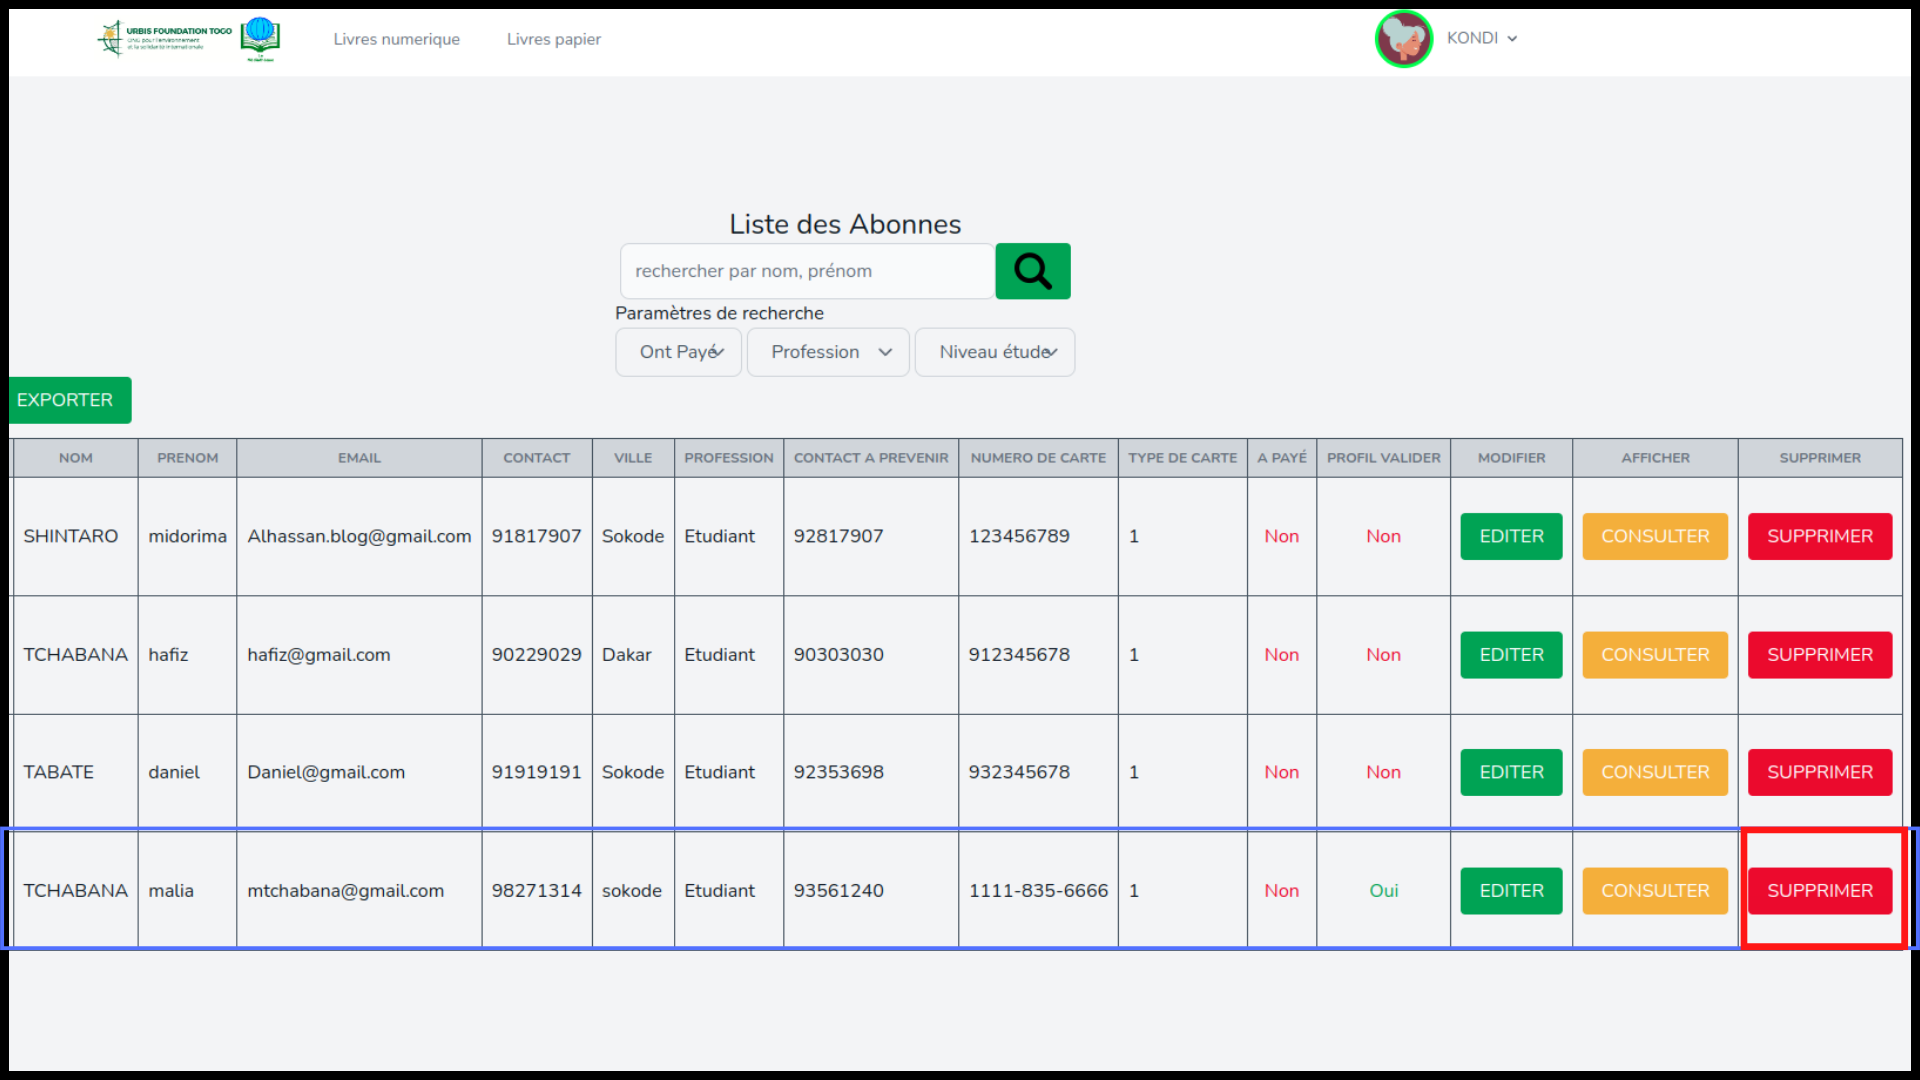
\includegraphics[scale=0.33]{img/abonne_delete.png}
\end{center}Un message de confirmation apparaît si vous souhait vraiment continuer cliquer encore sur \textbf{supprimer}. 
\begin{center}
\includegraphics[scale=0.56]{img/abonne_delete_confirm.png}
\end{center}
Vous constaterez que l'abonné aura belle et bien été supprimé.
\end{itemize}
\subsubsection{Sous menu \textbf{Abonnement}}
Ce sous menu permet de garder les traces des payements des abonnés pour leur
abonnement. Après avoir finis d'enregistrer un abonne, vous pouvez enregistrer le 
payement qu'il a effectuer pour l'abonnement (200 FCFA ou 500 FCFA). Pour le faire :
Cliquer sur le menu \textbf{Abonnement}. 
::::::::::::image requise::::::::::::\\
Vous verrez deux boutons : \textbf{Abonnement \& Annuler abonnement} et la liste des abonnement.\\
\begin{center}
\includegraphics[scale=0.56]{img/abonnements.png}
\end{center}
\textit{NB :} La colonne état permet de déterminer si l'abonnement est actif ou non.
\begin{itemize}
\item[•]  Cliquer sur \textbf{Abonnement}.
::::::::::::image requise::::::::::::\\
Sélectionner le nom et prénom de l'abonné. Le montant se calculera automatiquement.
\begin{center}
\includegraphics[scale=0.56]{img/abonnement_create.png}
\end{center}
Attendez que l'abonné vous paye puis cliquer sur le bouton enregistrer (si l'abonné ne paye pas on enregistre
pas son abonnement).\\
\begin{center}
\includegraphics[scale=0.56]{img/abonnements1.png}
\end{center}
Cela enregistrera l'opération comme vous pouvez le voir sur l'image ci dessus.
\item[•] Le bouton \textbf{Annuler abonnement} permet de faire expirer tous les abonnements.
\textbf{Vous devez le faire à chaque début d'année} cliquer dessus, un message d'alerte
ouvrira comme ceci.
\begin{center}
\includegraphics[scale=0.56]{img/abonnement_cancel.png}
\end{center}
confirmé en appuyant sur supprimer.Voici le résultat.
\begin{center}
\includegraphics[scale=0.56]{img/abonnements2.png}
\end{center}
\end{itemize}


\section{Import excel}
Pour enregistrer plusieurs livre papier ou numérique via une feuille excel, rendez vous sur le
tableau de bord puis sur le menu \textbf{Import excel}. Vous y verrez deux sous menu.
\textbf{Livre Papier et Livre numérique}.
\begin{itemize}
\item[•] Pour commencer choisissez le sous menu \textbf{Livre papier}. 
::::::::::::image requise::::::::::::\\
Une page s'ouvre. 
::::::::::::image requise::::::::::::\\
cliquer sur le bouton choisir un fichier.
::::::::::::image requise::::::::::::\\
Une onglet s'ouvre choisissez votre fichier excel.
::::::::::::image requise::::::::::::\\
Ensuit cliquer sur le bouton sélect.fichiers.
Une onglet s'ouvre la aussi choisissez le dossier contenant les images des livres inscrit dans le fichier
excel.
::::::::::::image requise::::::::::::\\
Puis appuyez sur le bouton importer. Après l'importation, vous serai redirigé vers la liste des ouvrages.

\textbf{NB:} Le fichier excel ne doit contenir qu'une seul feuille de calcul répondant
aux format çi dessous.\\
::::::::::Insérer format::::::::::
\end{itemize} 

\end{document}



